\documentclass[11pt, a4paper, bibliography=totoc]{report}
\usepackage{amsmath,amsthm,amssymb, ltablex, listings, enumerate, cancel, bussproofs, tabto, wasysym, algpseudocode, algorithm, savesym, mathtools, physics, xcolor, setspace, appendix, dirtree, ragged2e, graphicx, subcaption}
\usepackage[margin=3.5cm]{geometry}
\usepackage[font=footnotesize,labelfont=bf]{caption}
\usepackage[nottoc]{tocbibind} % adds Bibliography to TOCs
\usepackage[linktocpage]{hyperref}
\graphicspath{{./figures/}}

\hypersetup{
	colorlinks,
	linkcolor={red!50!black},
	citecolor={blue!50!black},
	urlcolor={blue!80!black}
}
\doublespacing
\pagestyle{headings}

% my math commands
\newcommand{\nats}{\mathbb{N}}
\newcommand{\reals}{\mathbb{R}}
\renewcommand{\P}[1]{\mathbb{P}\left( #1 \right) }
%\newcommand{\E}[1]{\mathbb{E} \left[ #1 \right] }
\newcommand{\E}[2]{\mathbb{E}_{#1} \left[ #2 \right] }
\newcommand{\V}[2]{\mathbb{V}ar_{#1} \left[ #2 \right]}
\newcommand{\KLD}[2]{\mathrm{KL} \left[ \left. \left. #1 \right|\right| #2 \right] }
\newcommand{\rp}{\hat{r}}
\newcommand{\expbuff}{\mathrm{E}}
\newcommand{\annbuff}{\mathrm{A}}
\newcommand{\repbuff}{\mathrm{D}}
\newcommand{\data}{\mathcal{D}}
\newcommand{\entropy}[1]{\mathbb{H} \left[ #1 \right] }
\newcommand{\MI}[1]{\mathbb{I} \left[ #1 \right] }
\newcommand{\w}{\mathbf{w}}
\newcommand{\x}{\mathbf{x}}
\newcommand{\y}{\mathbf{y}}
\newcommand{\thetab}{\pmb{\theta}}

% these commands are left over from my BBB report; I might never use them
\newcommand{\vfe}{\mathcal{F}(\data, \theta)}
\newcommand{\F}{\mathcal{F}}
\newcommand{\bepsilon}{\pmb{\epsilon}}
\newcommand{\bmu}{\pmb{\mu}}
\newcommand{\bsigma}{\pmb{\sigma}}
\newcommand{\btheta}{\pmb{\theta}}
\newcommand{\brho}{\pmb{\rho}}
\newcommand{\normal}[3]{\mathcal{N}(#1 \vert #2, #3)}

\newtheorem{claim}{Claim}
\newtheorem{theorem}{Theorem}
\newtheorem{lemma}{Lemma}
\newtheorem{hypothesis}{Hypothesis}
\newtheorem{corollary}{Corollary}
\newtheorem{proposition}{Proposition}
\newtheorem{definition}{Definition}
\newtheorem{assumption}{Assumption}
\newtheorem{example}{Example}

\begin{document}
\title{Active Reward Modelling for Agent Alignment}
\author{Sam Clarke}
\date{September 2019}
\renewcommand{\bibname}{References}
\maketitle

\begin{abstract} % ~200 words

\end{abstract}

\tableofcontents
% say somewhere around here about collaboration with Zac and Angelos
% and where do I say who my supervisor is?

\part{Background}

\chapter{Introduction}
Reinforcement Learning (RL) has made rapid progress in recent years at complex tasks such as playing Go \cite{silver2016mastering} and StarCraft II \cite{alphastarblog}. In their current form, the success of these systems relies on the objectives of the task being well-defined. Specifically, they require that the objectives can be expressed as a \textit{reward function}, which defines goals in terms of the reward associated with taking a given action when the world is in a given state. In the cases of Go and StarCraft, the game score function provides this.

However, real-world tasks lack such obvious reward functions. Therefore, if we aspire to use RL to assist us in the real-world, we need some other method of specifying our intentions. Put another way, we need to solve the \textit{agent alignment problem} \cite[p.~1]{Leike2018}:
\begin{quote}
	\textit{How can we create agents that behave in accordance with the user's intentions?}
\end{quote}

So far, systems have been developed which allow users to communicate their intentions by giving demonstrations and providing feedback (in the form of preferences or scalar rewards) on the agent's behaviour. For example, the \textit{inverse reinforcement learning} approach \cite{Ng2000, Ziebart2008} uses demonstrations by the user to infer their reward function. One can then use a standard RL algorithm to train an agent on the inferred reward function, to follow the user's intentions as expressed in the demonstrations. Alternatively, the \textit{RL from preferences} approach \cite{Christiano2017} queries the user for preferences about current agent behaviour, which it uses to learn the user's reward function and then refine the agent's behaviour accordingly, again by standard RL techniques.

These systems have been prototyped in simple domains, such as Atari games \cite{bellemare2013arcade} and simulated robotics tasks \cite{todorov2012mujoco}. However, the technology is far from mature. For example, the RL from preferences method requires on the order of thousands of user queries to learn to play simple Atari games, and so may struggle to scale to much more complex tasks. Indeed, an important property of any such system is to minimise the burden placed on the user. Clearly, there is no point in trying to automate some task if the automation procedure is even more demanding for the human than just performing the task themselves. In other words, we desire systems trained on user feedback to make sample efficient requests.

For this purpose, the RL from preferences method developed in \cite{Christiano2017} attempts to request only the most informative preferences from the user, a technique known as Active Learning (AL). However, the results of applying this technique were mixed; on some tasks, it showed improvement over requesting preferences uniformly at random, whilst for other tasks it made no significant difference, or even impaired performance. Accordingly, this component of the system was omitted the subsequent work by \cite{Ibarz2018}.

Our contribution is to conduct a detailed study into whether AL can be used to improve the efficiency of RL from user preferences, which we call \textit{active reward modelling}. Specifically, we test different hypotheses to explain the ambiguous results in \cite{Christiano2017}. We find that whether AL improves on the random acquisition of preferences depends on certain features of the environment and task, agreeing with the result in \cite{Christiano2017}. This environment-dependency is also consistent with state of RL in general, in which it is common for the success of algorithmic innovations on certain combinations of tasks and environments to fail to replicate when the task and environment are changed \cite{henderson2018deep}.

The dissertation is organised as follows. Part I lays out the relevant background material. All this material rests on an understanding of deep neural networks, which are explained in chapter 1. Chapter 2 outlines the basics of reinforcement learning. Chapter 3 concerns techniques for equipping deep neural networks with the ability to give estimates of the uncertainty in their output, which is used in Active Learning. These chapters provide only short overviews of entire research fields, but should be both self-contained and give sufficient detail to allow the reader to assess our contribution. Part II is concerned with our contribution. Chapter 5 explains our hypotheses for lack of success of active reward modelling in the previous work \cite{Christiano2017} and outlines the basic active reward modelling training protocol with which we our hypotheses. Chapter 6 details the experiments we performed to test our hypotheses, and the conclusions we drew from them. Chapter 7 summarises our contribution and suggests future work, as well as providing a critical evaluation and discussion of personal development and the relation of this dissertation to the material studied on the MSc course.

\chapter{Reinforcement Learning}
Reinforcement learning (RL) refers simultaneously to a problem, methods for solving that problem, and the field that studies the problem and its solution methods. The problem of RL is to learn what to do---how to map situations to actions---so as to maximise some numerical reward signal \cite[pp.~1-2]{Sutton2018}.

In this section we first introduce the elements of RL informally. We then formalise the RL Problem as the optimal control of incompletely-known Markov decision processes (finite? do I talk about PO?). We give a taxonomy of different RL solution methods and conclude with a description of one such method, Deep Q-Learning (DQN) that is of particular importance in this dissertation.

\section{Elements of Reinforcement Learning}
This subsection will introduce agent, environment, policy, reward signal, value function and [model] informally, similar to S\&B 1.3. Is this necessary or should I skip straight to the formalism?

\section{Finite Markov Decision Processes}
Finite Markov Decision Processes (finite MDPs) are a way of mathematically formalising the RL problem: they capture the most important aspects of the problem faced by an agent interacting with its environment to achieve a goal. We introduce the elements of this formalism: the agent-environment interface, goals and rewards, returns and episodes. Then...

\subsection{The Agent-Environment Interface} \label{subsection:agent_env_interface}
MDPs consist firstly of the continual interaction between an agent selecting actions, and an environment responding by changing state, and presenting the new state to the agent, along with an associated scalar reward. Recall that the agent seeks to maximise this reward over time through its choice of actions.

More formally, consider a sequence of discrete time steps, $t = 1,2,3, \dots$. At each time step $t$, the agent receives some representation of the environment's \textit{state}, $ S_t \in \mathcal{S} $, and chooses an \textit{action}, $ A_t \in \mathcal{A} $. On the next time step, the agent receives reward $ R_{t+1} \in \mathcal{R} \subset \reals $, and finds itself in a new state, $ S_{t+1} $. These interactions repeat over time, giving rise to a \textit{trajectory}, $ \tau $:
\begin{align*}
S_0, A_0, R_1, S_1, A_1, R_2, S_2, A_2, R_3, \dots
\end{align*}
% TODO insert Figure 3.1-like figure from S&B

A \textit{finite} MDP is one where the sets of states, actions and rewards are finite. In this case, the random variables $ S_t $ and $ R_t $ have well-defined discrete probability distributions which depend only on the preceding state and action. This allows us to define the \textit{dynamics} of the MDP, a probability mass function $ p : \mathcal{S} \times \mathcal{R} \times \mathcal{S} \times \mathcal{A} \mapsto [0,1] $, as follows. For any particular values $ s' \in \mathcal{S} $ and $ r \in \mathcal{R} $ of the random variables $ S_t $ and $ R_t $, there is a probability of these values occurring at time $ t $, given any values of the previous state $ s \in \mathcal{S} $ and action $ a \in \mathcal{A} $:
\begin{align*}
p(s', r \mid s, a) := \P{S_t = s', R_t = r \mid S_{t-1} = s , A_{t-1} = a }.
\end{align*}

A \textit{Markov} Decision Process is one where all states satisfy the Markov property. A state $ s_t $ of an MDP satisfies this property iff:
\begin{align*}
\P{s_{t+1}, r_{t+1} \mid s_t, a_t, s_{t-1}, a_{t-1}, \dots, s_0, a_0 } = \P{s_{t+1} \mid s_t, a_t}.
\end{align*}
This implies that the immediately preceding state $ s_t $ and action $ a_t $ are sufficient statistics for predicting the next state $ s_{t+1} $ and reward $ r_{t+1} $.

\subsection{Goals and Rewards}
The reader may have noticed that we first introduced MDPs as a formalism for an agent interacting with its environment to achieve a goal, yet have since spoken instead of maximising a reward signal $ R_t \in \reals $ over time. Our implicit assumption is the following hypothesis:
\begin{hypothesis}[Reward Hypothesis]
\textit{All of what we mean by goals and purposes can be well thought of as the maximization of the expected value of the cumulative sum of a received scalar signal (called reward).} \cite[p.~53]{Sutton2018}
\end{hypothesis}
However, this hypothesis gives no information about how to construct such a scalar signal; only that it exists. Indeed, recent work has shown that it is far from trivial to do so; possible failure modes include negative side effects, reward hacking and unsafe exploration \cite{Amodei2016}. This is central to the topic of this dissertation---our aim is to improve the sample efficiency of one particular method of reinforcement learning when the reward signal is unknown.

\subsection{Returns and Episodes} \label{rets_and_episodes}
Having asserted that we can express the objective of reinforcement learning in terms of scalar reward, we now formally define this objective. Consider the following objective:
\begin{definition}[(Future discounted) return]
Let a sequence of rewards between time step $ t + 1 $ and $ T $ (inclusive) be $ R_{t+1}, R_{t+1}, \dots, R_T $. Let $ \gamma \in [0, 1] $ be a discount factor of future rewards. Then we define the (future discounted) return of this sequence of rewards \cite[p.~57]{Sutton2018}:
\begin{equation} \label{G_t}
G_t := \sum_{k=0}^{\infty} \gamma^k R_{t+k+1}.
\end{equation}
\end{definition}

One reason for introducing a discount factor is because we would like this infinite sum to converge. Accordingly, we impose the condition that $ \gamma < 1 $ whenever the reinforcement learning task is \textit{continuous}, that is to say, there may be an infinite number of non-zero terms in the sequence of rewards $ \{R_{t+1}, R_{t+2}, R_{t+3}, \dots \} $.

The other kind of task is called \textit{episodic}. Here, interactions between the agent and environment occur in well-defined subsequences, each of which ends in a special \textit{terminal state}. The environment then resets to a starting state, which may be fixed or sampled from a distribution. To adapt the definition in (\ref{G_t}) to this case, we introduce the convention that zero reward is given after reaching the terminal state. This is because we typically analyse such tasks by considering a single episode---either because we care about that episode in particular, or something that holds across all episodes \cite[p.~57]{Sutton2018}. Observe that summing to infinity in (\ref{G_t}) is then identical to summing over the episode, and that the sum is well-defined regardless of the discount factor $ \gamma $.

\subsection{Policies and Value Functions} \label{policy_value_functions}
\textit{Policy} determines the behaviour of the agent. Formally, a policy $ \pi : \mathcal{S} \times \mathcal{A} \mapsto [0,1] $ defines a probability distribution over actions, given a state. That is to say, $ \pi(a \mid s) $ is the probability of selecting action $ a $ if an agent is following policy $ \pi $ and in state $ s $.

The \textit{state-value function} $ v_\pi : \mathcal{S} \mapsto \reals $ for a policy $ \pi $ gives the expected return of starting in a state and following that policy. More formally,
\begin{definition}[State-value function]
	Let $ \pi $ be a policy and $ s \in \mathcal{S} $ be any state. We write $ \E{\pi}{.}$ to denote the expected value of the random variable $ G_t $ as defined in (\ref{G_t}). Then the state-value function (or simply, value function) for policy $ \pi $ is:
	\begin{equation} \label{v_pi}
	v_\pi(s) := \E{\pi}{G_t \mid S_t = s} = \E{\pi}{\sum_{k=0}^{\infty} \gamma^k R_{t+k+1} \mid S_t = s}.
	\end{equation}
\end{definition}

The \textit{action-value function} $ q_\pi : \mathcal{S} \times \mathcal{A} \mapsto \reals $ for a policy $ \pi $ is defined similarly. It gives the expected return of starting in a state, taking a given action, and following policy $ \pi $ thereafter.
\begin{definition}[Action-value function]
	Let $ \pi $ be a policy, $ s \in \mathcal{S} $ be any state and $ a \in \mathcal{A} $ any action. Then the action-value function (or, Q-function) for policy $ \pi $ is:
	\begin{equation} \label{q_pi}
	q_\pi(s, a) := \E{\pi}{G_t \mid S_t = s, A_t = a} = \E{\pi}{\sum_{k=0}^{\infty} \gamma^k R_{t+k+1} \mid S_t = s, A_t = a}.
	\end{equation}
\end{definition}

\subsection{Optimal Policies and Optimal Value Functions} \label{optimal_policy_value_functions}
%TODO I'm confused about optimal policy. On Spinningup it seems to be defined as the policy that maximises the v_\pi(s_0). But S&B say it's the policy that maximises v_\pi(s) for all s \in S. These two defs are inconsistent bc consider an unreachable state? Spinningup def could say that some policy is optimal despite being bad in unreachable state; S&B def would not...
% http://spinningup.openai.com/en/latest/spinningup/rl_intro.html#the-rl-problem
% p.64 S&B
**Some words here based on the TODO above.
The problem of Reinforcement Learning is thus to find an optimal policy.

All optimal policies share the same value functions. We call these the \textit{optimal state-value function}, $ v_* $, and the \textit{optimal action-value function} $ q_* $:
\begin{definition}[Optimal state-value function (from {\cite[p.~62]{Sutton2018}})]
	$$ v_*(s)  := \max_\pi v_\pi(s) ~~ \forall s \in \mathcal{S} .$$
\end{definition}
\begin{definition}[Optimal action-value function (from {\cite[p.~63]{Sutton2018}})]
	$$ q_*(s,a)  := \max_\pi q_\pi(s,a) ~~ \forall s \in \mathcal{S} ~~ \forall a \in \mathcal{A} .$$
\end{definition}

There is a simple connection between optimal Q-function and optimal policy that will be used in Section \ref{RL_solution_methods}:
\begin{claim} \label{Q_claim}
	If an agent has $ q_* $, then acting according to the optimal policy when in some state $ s $ is as simple as finding the action $ a $ that maximises $ q_*(s,a) $ \cite[p.~64]{Sutton2018}.
\end{claim}

\subsection{Bellman Equations}
These value functions obey special recursive relationships called Bellman equations. The equations are proved by formalising the simple idea that the value of being in a state is the expected reward of that state, plus the value of the next state you move to. Each of the four value functions defined in Sections \ref{policy_value_functions} and \ref{optimal_policy_value_functions} satisfy slightly different equations. We prove the Bellman equation for the value function and state the remaining three for completeness.

\begin{proposition}[Bellman equation for $ v_\pi $ {\cite[p.~59]{Sutton2018}}]
	Let $ \pi $ be a policy, $ p $ the dynamics of an MDP, $ \gamma $ a discount factor and $ v_\pi $ a state-value function. Then:
	\begin{align}
		v_\pi(s) = \underset{\substack{a \sim \pi(. \mid s) \\ s', r \sim p(., . \mid s, a) }}{\mathbb{E}} \left[ r + \gamma v_\pi(s') \right]
	\end{align}
\end{proposition}
\begin{proof}
	\begin{align*}
		v_\pi(s) &:= \E{\pi}{G_t \mid S_t = s} \\
		         &= \E{\pi}{\sum_{k=0}^{\infty} \gamma^k R_{t+k+1} \mid S_t = s} \\
		         &= \E{\pi}{R_{t+1} + \gamma G_{t+1}} \\
		         &= \sum_{a \in \mathcal{A}} \pi(a \mid s) \sum_{\substack{s' \in \mathcal{S} \\ r \in \mathcal{R}}} p(s', r \mid s, a) \left[ r + \gamma \E{\pi}{G_{t+1} \mid S_{t+1} = s'} \right] \\
		         &= \sum_{a \in \mathcal{A}} \pi(a \mid s) \sum_{\substack{s' \in \mathcal{S} \\ r \in \mathcal{R}}} p(s', r \mid s, a) \left[ r + \gamma  v_\pi(s') \right] \\
		         &= \underset{\substack{a \sim \pi(. \mid s) \\ s', r \sim p(., . \mid s, a) }}{\mathbb{E}} \left[ r + \gamma v_\pi(s') \right]
	\end{align*}
\end{proof}

\begin{proposition}[Bellman equation for $ q_\pi $]
	Let $ \pi $ be a policy, $ p $ the dynamics of an MDP, $ \gamma $ a discount factor and $ q_\pi $ an action-value function. Then:
	\begin{align}
	q_\pi(s, a) = \underset{s', r \sim p(., . \mid s, a)}{\mathbb{E}} \left[ r + \gamma \underset{a' \sim \pi(.\mid s')}{\mathbb{E}}\left[q_\pi(s', a')\right] \right]
	\end{align}
\end{proposition}

\begin{proposition}[Bellman equation for $ v_* $ {\cite[p.~63]{Sutton2018}}]
	Let $ p $ be the dynamics of an MDP, $ \gamma $ a discount factor and $ v_* $ an optimal value function. Then:
	\begin{align}
	v_*(s) = \max_{a \in \mathcal{A}} ~ \underset{s', r \sim p(., . \mid s, a)}{\mathbb{E}} \left[ r + \gamma v_*(s') \right]
	\end{align}
\end{proposition}

\begin{proposition}[Bellman equation for $ q_* $ {\cite[p.~63]{Sutton2018}}] \label{bellman_q*}
	Let $ p $ be the dynamics of an MDP, $ \gamma $ a discount factor and $ q_* $ an optimal Q-function. Then:
	\begin{align}
	q_*(s, a) = \underset{s', r \sim p(., . \mid s, a)}{\mathbb{E}} \left[ r + \gamma ~ \underset{a' \in \mathcal{A}}{\max}\left[q_*(s', a')\right] \right]
	\end{align}
\end{proposition}

\section{Reinforcement Learning Solution Methods} \label{RL_solution_methods}
One method of solving the reinforcement learning problem is to explicitly solve a set of Bellman optimality equations. For example, in a finite MDP with $ n $ states and $ m $ actions, the Bellman equations for $ q_* $ are a set of $ n\cdot m $ equations in $ n\cdot m $ unknowns\footnote{This assumes that the agent can take any action in any state.}. Given the dynamics $ p $ of the MDP, standard techniques for solving systems of equations can be applied. Then, via Claim (\ref{Q_claim}), the agent has an optimal policy \cite[p.~64]{Sutton2018}.

However, in reality, we rarely have access to $ p $, or sufficient computational resources to solve this system of equations exactly \cite[p.~66]{Sutton2018}. Thus, much of the recent literature on RL solution methods focuses on finding approximate solutions.

In particular, there has been rapid development in a class of solution methods called \textit{deep reinforcement learning}. The idea is to use a \textit{deep neural network} to approximate some function that will yield an optimal policy. Typically, we approximate the optimal value function---this is called \textit{Q-learning}---or the optimal policy, directly---in which case it is termed \textit{policy optimization}\footnote{Some methods, such as DDPG \cite{lillicrap2015continuous}, TD3 \cite{fujimoto2018addressing} and SAC \cite{haarnoja2018soft} approximate both the optimal value function and the optimal policy.}.

In this section, we first provide background material on deep neural networks, necessary to understand how they approximate a Q-function or policy. We then explain in detail one particular deep reinforcement learning solution method, the deep Q-network, which is important for the rest of this thesis.

\subsection{Deep Neural Networks} \label{sec:dnn}
% model (func approx), data, loss, optimizer (mention batch GD, SGD, minibatch GD, then Adam and RMSProp briefly, since I use these)
% what is is relation between method of gradient descent and optimizer? where does the former fit into the  model, data, loss, optimizer thing? is it part of "optimizer"?
The goal of a deep neural network (NN) is to approximate some function $ f^* : \textbf{X} \mapsto \textbf{Y} $ \cite{Goodfellow-et-al-2016}. For example, in image classification, $ \textbf{X} $ may be image pixels, and $ \textbf{Y}Y $ some imge categories, for example, bird, plane or superhero. The neural network specifies a mapping $ y = f(\x ; \theta) $ that depends on some parameters $ \theta $. The task is then to learn the $ \theta $ that give the best approximation to the true function $ f^* $. A deep learning algorithm specifies how to do this.

As in machine learning in general, there are three key components to such an algorithm: model (or function approximator), cost function and optimization procedure andsubsubsection{Model}
The model, of course, is a deep NN. This simplest form of deep NN is a \textit{deep feedforward network}\footnote{They are also referred to as feedforward neural networks or multilayer perceptrons (MLPs)}. They are called feedforward because when the model is evaluated on input $ \x $, computation flows without ever feeding back into itself in a loop. They are called networks because it is natural to think of these models as being composed of many different functions, each of which is termed a \textit{layer}. Starting from the \textit{input layer}, the output of each layer flows into the next, through each of the \textit{hidden layers} until the \textit{output layer} is reaches and the function returns some value. Deep feedforward networks are deep inasmuch as they have many hidden layers \cite[p.~164]{Goodfellow-et-al-2016}.

\begin{example} \label{eg:nn}
Consider a very simple feedforward NN $ f : \reals^2 \mapsto \reals $ with one hidden layer. $ f $ is composed of three functions: $ f(\x) = f^{(3)}(f^{(2)}(f^{(1)}(\x))) $, where:
\begin{align*}
	f^{(1)}(\x) &= \mathbf{z} = \mathbf{W^1}\x \quad \text{for some $ 2\times 2 $ matrix $ \mathbf{W^1} $} \\
	f^{(2)}(\mathbf{z}) &= \mathbf{a} = \textup{ReLu}(\mathbf{a}) := \max\{0,\mathbf{a} \} \quad \text{where $ \max(.) $ is applied pointwise} \\
	f^{(3)}(\mathbf{a}) &= \mathbf{W^2}\mathbf{a} \quad \text{for some $ 1 \times 2 $ matrix $ \mathbf{W^2} $}
\end{align*}
\end{example}

\subsubsection{Cost function}
A \textit{cost function} (or \textit{loss function}) is some function that quantifies the performance of our model i.e. how close it is to the true function $ f^* $ we are trying to approximate. Most modern NNs use the \textit{negative log-likelihood} cost function\footnote{This is also referred to as the \textit{cross-entropy loss} function.} \cite[p.~138]{Goodfellow-et-al-2016}, which is simply the negative logarithm of the \textit{likelihood function}. Given a parametric family of probability distributions $ p_{\text{model}}(\x ; \theta) $ over the same space, a likelihood function gives the probability of a set of observations for different settings of the model parameters $ \theta $. More formally, consider a set of $ m $ i.i.d. examples $ \mathbb{X} = \{\x_1, \dots, \x_m \} $ drawn from a true but unknown data generating distribution. Then the likelihood function $ L(\theta) $ is defined by:
\begin{align*}
L(\theta) :=&~ p_{\text{model}}(\mathbb{X} ; \theta) \\
	=&~ \Pi_{i=1}^m p_{\text{model}}(\x_i ; \theta)
\end{align*}
Taking the logarithm of this function improves numerical stability, and taking its negative value is a convention because optimization in machine learning typically means \textit{minimizing} some function. Finally, we can divide by $ m $, which shows how we can interpret this function cost function as an expectation with respect to the empirical distribution $ \hat{p}_{\text{data}} $ defined by the training data $ \mathbb{X} $. Notice that minimising this modified function will give the same result and maximising the likelihood. So, we define the negative log likelihood cost function $ \text{NLL}(\theta) $ as
\begin{align} \label{eq:nll}
\text{NLL}(\theta) :=& -\frac{1}{m} \log L(\theta) \nonumber \\
=& -\frac{1}{m} \sum_{i=1}^m \log p_{\text{model}}(\x_i ; \theta) \nonumber \\
=&  -  \E{\x \sim \hat{p}_\text{data}}{\log p_{\text{model}}(\x ; \theta) } 
\end{align}
and seek the parameters $ \theta_{\text{ML}} $ which minimise this function:
\begin{align}
{\theta}_{\text{ML}} :=&{\arg\min}_{\theta} \text{NLL}(\theta) \nonumber
\end{align}

In this thesis, we will use $ \text{NLL}(\theta) $ cost function. Our model $ p_{\text{model}} $ is some neural network. Importantly, the NN output must define a probability distribution, which is implemented by making its final layer a softmax or Gaussian probability density function, for categorical and real-valued data, respectively. Furthermore, we actually use a slight generalisation of this procedure to estimate a conditional probability  $ p_{\text{model}}(\y \mid \x; \theta ) $ where $ \x \in \mathbf{X} $ are some inputs and $ \y \in \mathbf{Y} $ some outputs (also called \textit{targets}) of the function $ f^* : \textbf{X} \mapsto \textbf{Y} $ we are trying to approximate. This setting is called \textit{supervised learning}, because the training data is a set of supervised examples i.e. pairs of inputs and correctly labelled outputs. Finally, note that in the real-valued case, using a Gaussian density function on the output of a NN is equivalent to not passing the output values through the density function, and instead simply minimising $ \frac{1}{m} \sum_{i=1}^{m} ( \hat{y}_i - y_i ) $, the mean squared error between the inputs and targets  over the training data $ \langle (\x_i, y_i) \rangle_{i=1}^m $ where $ \hat{y_i} = f(\x_i) $, our model's prediction for input $ \x_i $ \cite[p.~132]{Goodfellow-et-al-2016}.

%Our data (as we shall see) will be generated by an RL agent acting in an environment, and by querying an oracle for preferences about that agent's behaviour. We will optimize the loss function using Adam.

%TODO do I use weight decay? If so, need to include this paragraph
%The cost function may include additional terms, for example those which add \textit{regularisation}. Such terms discourage the model parameters from simply memorising the training data, which would lead to poor generalisation to unseen examples. One simple example is including a \textit{weight decay} term, which modifies Equation \ref{eq:nll} to:
%\begin{equation} \label{eq:nllwd}
%\theta_{\text{ML}} := {\arg\min}_{\theta} ~ \lambda \left\lVert \theta \right\rVert^2_2 - \sum_{i=1}^{m} p_{\text{model}}(\x_i ; \theta)
%\end{equation}

\subsubsection{Optimization procedure}
The third component of a deep NN algorithm is the \textit{optimization procedure}. This specifies how we use the cost function to update the NN parameters $ \theta $. Since NNs of interest are typically non-convex functions (due to non-linear layers such $ f^{(2)} $ in Example \ref{eg:nn}), Equation \ref{eq:nll} cannot be optimized in closed form. Thus, we require some numerical optimization procedure \cite[p.~151]{Goodfellow-et-al-2016}; the most common is some variation of \textit{gradient descent}.

Gradient descent works by computing $ \nabla_\theta L(\theta) $, the partial derivate of some cost function $ L(\theta) $ with respect to the model parameters $ \theta $. Since the partial derivate of a function points in the direction of steepest ascent, selecting a new set of parameters $ \theta' = \theta - \epsilon ~ \nabla_\theta L(\theta) $ will mean that $ L(\theta') $ is less than $ L(\theta) $ for some small enough $ \epsilon $ \cite[p.~83]{Goodfellow-et-al-2016}. We can iteratively perform this procedure and eventually reach a \textit{local minimum} i.e. a point where $ L(\theta) $ is lower than at all neighbouring points. $ \epsilon $ is called the \textit{learning rate}; it is typically chosen by trying several small values and choosing that which results in the lowest final $ L(\theta) $.

If $ L(\theta) $ is non-convex then there is no guarantee that this point will be a \textit{global minimum} i.e. a point where $ L(\theta) $ takes its lowest possible value. Much machine learning research is concerned with modifications to this procedure, and how to set initial parameter values in order to avoid getting stuck in local minimum that lead to poor performance. As it turns out, finding local minima that are low enough often leads to very good performance.

One important modification is called \textit{stochastic gradient descent} (SGD). Notice that minimising Equation \ref{eq:nll} via gradient descent requires computing
\begin{align*}
\nabla_\theta \text{NLL}(\theta) = \frac{1}{m} \nabla_\theta \sum_{i=1}^{m} - \log p_{\text{model}}(\x_i ; \theta)
\end{align*}
on each iteration, which has computational complexity $ O(m) $ \cite[p.~149]{Goodfellow-et-al-2016}. For large training sets, this is infeasible.

SGD is based on the simple idea that this gradient is an expectation over the training data which we can approximate using a small sample \cite[p.~149]{Goodfellow-et-al-2016}:
\begin{equation}
\nabla_\theta \text{NLL}(\theta) \approx \frac{1}{m'}  \nabla_\theta \sum_{i=1}^{m'} - \log p_{\text{model}}(\x_i ; \theta)
\end{equation}
for some $ \mathbb{B} = \{\x_1, \dots, \x_{m'} \} \subset \mathbb{X} $ called a \textit{minibatch}, sampled uniformly at random from $ \mathbb{X} $.

In this thesis, we use a further variant of SGD called \textit{RMSProp} \cite{tieleman2012lecture}. This maintains individual learning rates for each model parameter and adapts them individually. Specifically, on each learning update, parameter $ \theta_i $ is rescaled according to the inverse square root of an exponentially weighted moving average of the historical squared values of the partial derivate of the cost function with respect to $ \theta_i $. This results in larger learning updates for parameters with small partial derivatives, and smaller learning updates for parameters with larger partial derivates. The intention is to converge to a minimum more rapidly than SGD. Algorithm \ref {alg:rmsprop} gives the precise procedure \cite[p.~304]{Goodfellow-et-al-2016}. 
\begin{algorithm}
	\caption{RMSProp.}
	\label{alg:rmsprop}
	\begin{algorithmic}[1]
		\Require Global learning rate $ \epsilon $, decay rate $ \rho $, initial parameters $ \theta $
		\State Initialise $ \mathbf{r} = 0 $ to accumulate squared gradients for each parameter
		\Repeat
		\State Sample minibatch $ \mathbb{B} = \{\x_1, \dots, \x_{m'} \} $
		\State Compute gradient $ \mathbf{g} \gets \frac{1}{m} \nabla_\theta \sum_i \text{NLL}(\x_i ; \theta) $
		\State Accumulate squared gradient $ \mathbf{r} \gets \rho \mathbf{r} + (1-\rho) {g} \odot \mathbf{g}  $
		\State Update parameters: $ \theta \gets \theta - \frac{\epsilon}{\sqrt{r + 10^{-6}}}\odot \mathbf{g} $
		\Until{convergence}
	\end{algorithmic}
\end{algorithm}
Note that the operations on lines 4-6 are all applied element-wise (that is, to each parameter individually). The adding $ 10^{-6} $ to $ r $ on line 6 improves numerical stability.

\subsection{Deep Q-network} \label{DQN}
We now have the necessary background to explain the deep Q-network (DQN). The idea is simply to use a deep NN to approximate the optimal Q-function $ q_* $ using a deep neural network $ Q(s,a; \theta) $ as the function approximator \cite{Mnih2015}. The agent-environment interactions yield experience $\langle (s_t, a_t, r_{t+1}, s_{t+1}) \rangle_{t=0}^T $ which can be used as training data. We can then simply perform gradient descent on the parameters $ \theta_i $ at iteration $ i $ to reduce the mean squared error between predictions $ Q(s,a; \theta_i) $ and targets given by the Bellman equation for $ q_*(s,a) $, from Proposition \ref{bellman_q*}. Since we do not have access to the true value of these targets, we instead use approximate target values $ y = r + max_{a'} ~ Q(s', a' ; \theta_i^-) $, with $ \theta_i^- $ some previous network parameters.

So far, this looks very similar to the supervised learning setting. However, there are three important differences that come with reinforcement learning. There are two sources of serrelations: both (i) in the data set, and (ii) between $ Q(s,a ; \theta_i) $ and the targets. AlsoFurti) updates to $ Q $ may change the policy and thus change the data distribution. This leads to instability in training. To address this, the authors propose two algorithmic innovations. Firstly, instead of training on experience in the order that it is collected, the agent maintains a buffer of experience $ D_t = \{ e_1, e_2, \dots, e_t \} $ where $ e_t = (s_t, a_t, r_{t+1}, s_{t+1}) $. When making learning updates, drawing minibatches uniformly at random from this buffer breaks correlations in the experience sequence and smooths over changes in the data distribution, alleviating problems (i) and (iii). This is termed \textit{experience replay}. Secondly, to reduce correlations between $ Q $ and the targets and alleviate problem (ii), the approximate target values are updated to match the parameters $ Q $ only every $ C $ steps for some hyperparameter $ C > 1 $.

With these changes, we arrive at a loss function $ \ell_i(\theta_i) $ for each learning update $ i $:
\begin{align*}
\ell_i(\theta_i) &= \E{ s,a,r }{ (\E{s'}{y \mid s,a} - Q(s,a;\theta_i))^2 } \\
                 &= \E{ s,a,r }{ \E{s'}{y - Q(s,a;\theta_i) \mid s,a } ^2 } \\
                 &= \E{ s,a,r }{ \E{s'}{(y - Q(s,a;\theta_i))^2 \mid s,a}  - \V{s'}{y - Q(s,a;\theta_i)) \mid s,a}   } \\
                 &= \E{s,a,r,s'}{(y - Q(s,a;\theta_i))^2} - \E{s,a,r}{\V{s'}{y}}
\end{align*}
where the expectations and variances are with respect to samples from the experience replay. This loss function is then optimized by stochastic gradient descent with respect to the network parameters $ \theta_i $. Note that the final term is independent of these parameters, so we can ignore it. Finally, the authors found that stability is improved by clipping the error term $ y - Q(s,a;\theta_i) $ to be between $ -1 $ and $ 1 $.

We summarise this training procedure in Algorithm \ref{alg:dqn}. To ensure adequate exploration, the agent's policy is $ \epsilon $-greedy with respect to the current estimate of the optimal action-value function.

\begin{algorithm}
	\caption{Deep Q-learning with experience replay.}
	\label{alg:dqn}
	\begin{algorithmic}[1]
		\State Initialise replay memory $ D $ to capacity $ N $
		\State Initialise neural network $ Q $ with random weights $ \theta $ as approximate optimal action-value function
		\State Initialise neural network $ \hat{Q} $ with identical weights $ \theta^- = \theta $ as approximate target action-value function
		\State Reset environment to starting state $ s_0 $
		\For{$ t=0, \dots, T $}
		\State With probability $ \epsilon $ execute random action $ a_t $
		\State otherwise execute action $ a_t = \arg\max_a Q(s_t, a ; \theta) $
		\State Observe next state and corresponding reward $ s_{t+1}, r_{t+1} \sim p(.,.\mid s_t,a_t) $
		\State Store transition $ (s_t, a_t, r_{t+1}, s_{t+1}) $ in $ D_t $
		\State Randomly sample minibatch of transitions $ (s_j, a_j, r_{j+1}, s_{j+1}) \sim D_t $
		\State Set $ y_j = \begin{cases}
		                   r_{j+1} \text{ if episode terminates at step $ j+1 $} \\
		                   r_{j+1} + \gamma \max_{a'} \hat{Q}(s_{j+1}, a_j ; \theta^- ) \text{ otherwise}
		\end{cases}$
		\State Do gradient descent on $ (y_j - Q(s_j, a_j ; \theta))^2 $ w.r.t network parameters $ \theta $
		\State Every $ C $ steps set $ \theta^- = \theta $
		\EndFor
	\end{algorithmic}
\end{algorithm}

Note that line 11 assumes we are training DQN to perform an episodic task, hence the first case which follows the convention given in Section \ref{rets_and_episodes} whereby zero reward is given for all states after the terminal state. If the task were instead continuing, line 11 would simply be $ y_j = r_{j+1} + \gamma \max_{a'} \hat{Q}(s_{j+1}, a_j ; \theta^- ) $.

\section{Reinforcement Learning from Unknown Reward Functions}
So far, we have assumed that as the agent interacts with the environment, it receives both information about the next state and the associated scalar reward. This presents an obvious challenge if we want to apply RL to solve real-world problems: since the world does not give scalar rewards, it seems we would have to manually specify a reward function mapping states of the world to rewards. For complex or poorly defined goals, this is difficult to do. If we try instead to design an approximate reward function, an agent optimizing hard for this objective will do so at the expense of satisfying our preferences \cite[p.~1]{Christiano2017}.

To circumvent this issue, a growing body of work studies how to do RL from various forms of human \textit{feedback}, instead of an explicit reward function. Three main feedback methods have been studied, all of which involve a human-in-the-loop providing information to the agent about the desired behaviour. Firstly, an agent may learn from expert demonstrations. This may involve using demonstrations to infer a reward function, an approach known as \textit{inverse reinforcement learning} \cite{Ng2000, Ziebart2008}. One can then use a standard RL algorithm on this recovered reward function. Other methods involve training a policy directly from demonstrations, referred to as \textit{imitation learning} \cite{Ho2016, Hester2017}.

Secondly, an agent may learn from feedback on its current policy in the form of scalar rewards \cite{Knox2009, Warnell2017}. Instead of providing a set of demonstrations, the human-in-the-loop observes the agent's behaviour and gives an appropriate reward. If it is assumed that the human provides this reinforcement according to some latent reward function $ \hat{r} : \mathcal{S} \times \mathcal{A} \mapsto \reals $, then standard supervised learning techniques can be applied to model this function. The agent can then select actions so as to maximise expected modelled reward. This approach differs from manually specifying a reward function because the human does not provide a precise function mapping all possible state-action pairs to rewards in advance. Rather, the human remains in the loop, providing reinforcement to the agent in an online fashion.

Finally, an agent may learn from binary preferences over trajectories \cite{Wilson2012, Christiano2017}. As with the \textit{policy feedback} method, the human-in-the-loop observes the agent's behaviour. However, instead of giving reinforcement in the form of scalar rewards, they are periodically presented with a pair of trajectories and must indicate which they prefer\footnote{The human also has the option of expressing indifference, or that the trajectories are incomparable.}. Given some assumptions about how the human's preferences relate to their latent reward function, we can again model $ \hat{r} $ by supervised learningI Then, standard RL algorithms can be applied to maximise the cted $ \rp $ over time.
%TODO highlight that Warnell doesn't do RL, but rather the agent just selects actions to maximise \rp? I'm confused about why this works. If you don't apply an RL algo, won't the agent be too myopic?
%TODO is this last paragraph too specfic since it only applies to the reward learning from trajectory preferences in the Deep RL case?

Each of these methods have shown promising results, and some of the advantages and disadvantages are summarised in Table \ref{table:1}.

\small\singlespacing\RaggedLeft
\begin{tabularx}{\textwidth}{ 
		|X|X|X|X|
	}
	\hline 
\textbf{Property} & \textbf{Trajectory preferences} & \textbf{Expert demonstrations} & \textbf{Policy feedback} \\ 
\hline 
Demandingness for human & Human only needs to judge outcomes & Human needs to perform task (expertly) & Human needs to provide suitable scalar rewards \\ 
\hline 
Upper bound on performance? & Superhuman performance is possible & Impossible to significantly surpass performance of expert & Superhuman performance is possible \\ 
\hline 
Suitability to exploration-heavy tasks & Limited\footnote{\label{footnote:exploration}The human can only give feedback on states visited by the agent. If the agent does not explore well, this limits the amount of information the human can convey. Since exploration is determined by the inferred reward func } & Well suited, since demonstrations can guide exploration & Limited\footnote{See footnote \ref{footnote:exploration}} \\ 
\hline 
Communication efficiency & On the order of hundreds of bits per human hour & Much richer in information than trajectory preferences \footnote{\cite{Ibarz2018} show that demonstrations half the amount of human time required to achieve the same level of performance} & Scalar rewards provide richer information than binary preferences over trajectories, but not as rich as demonstrations \\ 
\hline 
Computational efficiency (in simple Atari environments) & On the order of 10 million RL time steps & On the order of 10 million RL time steps & On the order of thousands of learning time steps \footnote{Note that the work which prototypes this method trains, with an unspecified amount of compute, a deep autoencoder to extract 100 features from the Atari game screen \textit{before} commencing the RL stage. The other methods do not do such pretraining, thus the reported results do not allow for a fair comparison.} \\ 
\hline
\caption{Summary of the properties of using different forms of human feedback in RL without a reward function.} \label{table:1}
\end{tabularx}
\normalsize\doublespacing\justify

Noticing that the properties on which learning from preferences performs poorly are precisely those on which learning from demonstrations performs well, it is intuitive to think that a combination of feedback methods will give better performance than either one individually. Recent work has confirmed this intuition. Specifically, \cite{Ibarz2018} test this method on nine Atari games \cite{bellemare2013arcade}, and show that combined preferences and demonstrations outperform only demonstrations on eight games, and only preferences on the four exploration-heavy games\footnote{The contribution of demonstrations in games without difficult exploration is not significant, except for in two games where demonstrations are harmful compared to using only preferences. The authors hypothesise that this is due to the relatively poor performance of the expert \cite[p.~6]{Ibarz2018}}. \cite{Palan2019} show that in a 2D driving simulator \cite{Byk2017} and two OpenAI Gym environments \cite{brockman2016gym}, using just one expert demonstration reduces by a factor of 3 the number of human preferences required to achieve the same performance \cite[p.~6]{Palan2019}.

This dissertation concerns using active learning to improve the performance of reward learning from trajectory preferences. So far, work on feedback from preferences has taken two different approaches: training a reward model on handcrafted features of the environment, and taking the deep learning approach of training a reward model end-to-end without handcrafted features. As active learning has already been shown to improve performance in the former setting \cite{Byk2017}, we focus on applying active learning in the latter setting. Algorithmic innovation in this setting is also more exciting, because if we want to scale RL to real-world tasks, it is unlikely that we will be able to handcraft all the correct features.

In the remainder of this section, we explain in detail the algorithm used for the latter approach, which was developed in \cite{Christiano2017}. We then summarise briefly the difference in learning from preferences with handcrafted features, in which active learning has already been applied successfully.

\subsection{Reward Learning from Trajectory Preferences in Deep RL}

\subsubsection{Setting}
The agent-environment interface is as described in Section \ref{subsection:agent_env_interface}, with the modification that on step $ t $, instead of receiving reward $ R_{t+1} \in \mathcal{R} \subset \reals $, there is an \textit{annotator} who expresses preferences between \textit{trajectory segments}, or \textit{clips}. A clip is a finite sequence of states and actions $ ((s_0,a_0), (s_1,a_1),\dots,(s_{k-1},a_{k-1})) \in (\mathcal{S} \times \mathcal{A})^k $. If the annotator prefers some clip $ \sigma^1 $ to another clip $ \sigma^2 $, write $ \sigma^1 \succ \sigma^2 $. The annotator may also be indifferent between the clips, in which case we write $ \sigma^1 \sim \sigma^2 $. The agent does not see the annotator's implicit reward function $ r : \mathcal{S} \times \mathcal{A} \mapsto \mathcal{R} $, and must instead use the preferences expressed by the annotator to maximise $ r $ over time. This is the goal of reward learning from trajectory preferences.
%TODO need to define \succ in terms of r(.,.) ?
If the annotator could write down their true $ r $, then clearly we could perform traditional RL instead of taking the reward learning approach. However, as we noted above, we are interested in applying RL to tasks for which we do not have the true $ r $, which is when reward learning is useful. Nonetheless, for the purposes of quantitatively evaluating the method, we consider tasks for which we do have access to the true $ r $.

\subsubsection{Method}
The method has two components: a policy $ \pi : \mathcal{S} \times \mathcal{A} \mapsto [0,1] $ and an estimate of the annotator's reward function, $ \rp : \mathcal{S} \times \mathcal{A} \mapsto \mathcal{R} $, called a \textit{reward model} or \textit{reward predictor}. Both components are parametrised by a deep neural network. The agent learns to maximise the annotator's implicit reward function over time by iterating through the following three processes:
\begin{enumerate}
	\item Reinforcement learning by a traditional deep RL algorithm whereby policy $ \pi $ interacts with the environment for $ T $ steps and updates its parameters to optimise $ \rp $ over time. Agent experience $ \expbuff = ((s_0, a_0), (s_1, a_1),\dots, (s_{T-1}, a_{T-1}) ) $ is stored.
	\item Select pairs of clips $ (\sigma^1, \sigma^2) $ from $ \expbuff $, request a preference $ \mu $ from the annotator on each sampled pair, and add the labelled pair to the annotation buffer $ \annbuff $.
	\item Supervised learning to train the reward model on $ \annbuff $, the preferences expressed by the annotator so far.
\end{enumerate}
More detail on each process is provided below.

\subsubsection{Process 1: Training the policy}
As mentioned, process 1 is akin to traditional RL except $ \rp $ is used in place of the environment reward $ r $. There are two subtleties to mention. Firstly, since $ \rp $ is learned while RL is taking place, \cite{Christiano2017} prefer policy optimization methods over Q-learning, as these have been successfully applied to RL tasks with a non-stationary reward function \cite{Ho2016}. Specifically, they use A2C \cite{Mnih2016} and TPRO \cite{Schulman2015}. However, the follow up paper \cite{Ibarz2018} uses a Q-learning method\footnote{The reason for deviating from the recommendation in \cite{Christiano2017} is that \cite{Ibarz2018} combine reward learning from trajectory preferences and expert demonstrations, and DQfD is state-of-the-art for the latter problem.}, DQfD \cite{Hester2017}, and it is not clear that performance is impaired. Hence, the literature is ambiguous on whether a non-stationary reward function is necessarily problematic for Q-learning. %TODO link to the section of my method where I say that I used DQN; motivate why I did this; say that reinitialising agent should make it okay.

Secondly, since the reward model $ \rp $ is trained only on pairwise comparisons, its scale is underdetermined. Previous work therefore proposes periodically normalising $ \rp $ to have zero mean and constant standard deviation over the examples in $ \annbuff $. This is crucial for training stability since deep RL is sensitive to the scale of rewards. %TODO perhaps comment here or later on what Zac said that scaling rewards can actually in some cases change optimal policy...
%TODO comment here on later on the subtelties of normalisation when using an ensemble for your rewards.

\subsubsection{Process 2: Selecting and annotating clip pairs}
Previous work uses two methods for selecting clip pairs. \cite{Ibarz2018} sample uniformly at random from $ \expbuff $. \cite{Christiano2017} train an ensemble of three reward predictors and select the clip pairs with the maximum standard deviation across the ensemble. Roughly this favours clip pairs on which the model is most uncertain, with the hope of improving sample efficiency (that is to say, being able to learn $ \rp $ with fewer labels from the annotator). However, they found that relative to random selection, this sometimes impaired performance and slowed down training. In Section ** we consider what caused this.

The selected clip pairs $ \sigma^1, \sigma^2 $ are then annotated with a label $ \mu $, indicating which clip is preferred. $ \mu $ is a distribution over $ \{1,2\} $ where $ \mu(1) = 1, \mu(2) = 0 $ if $ \sigma^1 \succ \sigma^2 $; $ \mu(1) = 0.5, \mu(2) = 0.5 $ if $ \sigma^1 \sim \sigma^2 $; or $ \mu(1) = 0, \mu(2) = 1 $ if $ \sigma^2 \succ \sigma^1 $. The triples $ (\sigma^1, \sigma^2, \mu) $ are then added to $ \annbuff $. The majority of previous work uses a \textit{synthetic annotator} rather than an actual human. Labels are simply generated according to the (hidden) ground truth reward function $ r $, where $ \sigma^1 \succ \sigma^2 $ if $ \sum_t r(s_t^1, a_t^1) > \sum_t r(s_t^1, a_t^1) $; $ \sigma^1 \sim \sigma^2 $ if $ \sum_t r(s_t^1, a_t^1) = \sum_t r(s_t^1, a_t^1) $; and $ \sigma^2 \succ \sigma^1 $ otherwise. This facilitates quicker experimentation and more clear performance metrics (by using hidden ground truth reward function to evaluate agent performance and reward model alignment).

\subsubsection{Process 3: Training the reward model}
The training of $ \rp $ is based on the following assumption:
\begin{assumption} \label{assumption:1}
	The annotator's probability of preferring clip 1 to clip 2, $ \hat{P}(\sigma^1 \succ \sigma^2) $, depends exponentially on the value of $ \hat{r} $ summed over the clips.
\end{assumption}
This allows us to write:
\begin{equation} \label{eq:softmax}
\hat{P}(\sigma^1 \succ \sigma^2 ; \rp) = \frac{\exp \sum_t \hat{r}(s_t^1, a_t^1)}{\exp \sum_t \hat{r}(s_t^1, a_t^1) + \exp \sum_t \hat{r}(s_t^2, a_t^2)}
\end{equation}
We can then fit the parameters of $ \rp $ by treating the problem as binary classification. In other words, we can use standard supervised learning techniques to optimize the parameters of $ \rp $ so as to minimise the cross-entropy loss between the predictions in \ref{eq:softmax} and the annotator's labels.
\begin{equation} \label{eq:loss}
\text{loss}(\hat{r}) = -\sum_{(\sigma^1, \sigma^2, \mu) \in \annbuff} \mu(1) \log \hat{P}(\sigma^1 \succ \sigma^2 ; \rp) + \mu(2)\log \hat{P}(\sigma^2 \succ \sigma^1 ; \rp)
\end{equation}
Assumption \ref{assumption:1} follows the Elo rating system developed for chess \cite{elo1978rating}. Given a zero-sum game and two players with a scalar rating, Elo specifies a mapping from player ratings (in our case: reward) to the probability of each player winning (in our case: the probability of each clip being preferred by the annotator).

\subsection{Reward Learning from Trajectory Preferences with Handcrafted Feature Transformations}
\subsubsection{Setting}
\cite{Byk2017} consider a more narrow setting. There are two vehicles, $ H $ which is ``human driven'', and $ R $ which is a ``robot''. The vehicles are in a 2D environment with each obeying a simple point-mass dynamics model, with state space $ \mathcal{S} $:
\begin{align*}
[ \dot{x}~~~ \dot{y}~~~ \dot{\theta} ~~~ \dot{v} ] = [  v \cdot \cos(\theta) ~~~ v \cdot \sin(\theta) ~~~ v \cdot u_1 ~~~ u_2 - \alpha\cdot v  ] 
\end{align*}
where $ v $ and $ \theta $ are vehicle velocity and direction respectively. The action space $ \mathcal{A} $ is $ [u_1, u_2] $ which represent steering and acceleration respectively. $ \alpha $ is a friction coefficient.

They assume that $ \hat{r} : \mathcal{S} \times \mathcal{A} \mapsto \reals $ is a linear combination of a set of five features:
\begin{align*}
\rp(s,a) = \w^T \phi(s,a).
\end{align*}
These five features $ \w = [w_1, w_2, w_3, w_4, w_5] $ are handcrafted, and correspond to (i) distance to road boundary, (ii) distance to centre of road lane with an extra penalty for shifting lane, (iii) difference between vehicle speed and the speed limit, (iv) dot product between $ \theta $ and a vector pointing along the road, and (v) a non-spherical Gaussian over the distance from $ R $ to $ H $ (to penalise collisions).

Like \cite{Christiano2017}, there is annotator who is queried for preferences on trajectory segments. Some $ \w_\text{true} $ is specified in advance, and the annotator uses this to answer the queries as in Process 2 of \cite{Christiano2017}.

\subsubsection{Method}
\cite{Byk2017} do not attempt to train a policy using the learned reward model. Their performance metric is simply the expected similarity of the true and predicted feature weights:
\begin{align*}
m = \mathbb{E}\left[  \frac{\w \cdot \w_\text{true}}{\vert \w \vert \vert \w_\text{true} \vert}  \right]
\end{align*}
They generate queries by solving a constrained optimization problem to find the two trajectory segments that will maximise the volume removed from the hypothesis space. Using the same mapping from reward space to preference space as \cite{Christiano2017} (Equation \ref{eq:softmax}), they start with a uniform prior over the space of all $ \w $ (uniform over the unit ball), generate a query, get a preference from the annotator, and perform a Bayesian update on this labelled clip pair. Thanks to the simple function form of their reward model, this Bayesian update has a closed form solution. They repeat this procedure until the reward model is close to the true reward function, according to $ m $.

\chapter{Uncertainty in Deep Learning}
If we are to use deep NNs for practical applications, it is crucial that they output not only point estimates, but also their uncertainty in those estimates. For example, suppose a deep NN is being used to drive an autonomous vehicle. If it encounter a situation in which it is uncertain about whether to brake or not, we probably want it to hand over control to a human driver, rather than blindly taking its best guess. Equally, if a deep NN is being used for medical diagnosis and is confronted with an unfamiliar stimulus, it should request more data or alert a human doctor. In Section \ref{sec:dnn}, we explained that NNs output probability distributions. For example, with categorical data, the final layer of the network is typically a softmax function, which gives the probability of the input being in each of the possible classes. However, such probability distributions do not in fact accurately reflect uncertainty \cite[p.~13]{Gal2017a}.

In this chapter we first summarise some of the techniques used equip NNs with the ability to output uncertainty estimates alongside point estimates. We then explain how such uncertainty estimates can be applied to the problem of Active Learning (AL), which is central to the topic of this dissertation.

\section{Bayesian Neural Networks}
Bayesian neural networks (BNNs) different from standard NNs in that they maintain a distribution over their weights rather than single values. As in all of machine learning, we then require an algorithm for learning from data. The mathematically correct way to do this for BNNs is to perform Bayesian inference on the weights on the network, i.e. compute a posterior distribution over the weights, given the training data. Then, given the posterior distribution over weights, to answer predictive queries we take expectations under this distribution:
\begin{align*}
P(\hat{y} \mid \hat{x}) = \E{ P(w|D) }{P(\hat{y} \mid \hat{x}, w) }
\end{align*}
However, this method of inference is intractable for the size of models that deep learning uses. Instead, we need to find an approximation to the true posterior.

Variational Inference (VI) is one such approximation method. Historically, many of the attempts to perform VI on BNNs were not particularly practical. For example, one algorithm, Bayes by Backprop \cite{Blundell2015}, requires doubling the number of model parameters, making training more computationally expensive, and is very sensitive to hyperparameter tuning. However, recent techniques allow almost any network trained with a stochastic regularisation technique, such as dropout, to, given an input, obtain a predictive mean and variance (uncertainty), without any complicated augmentation to the network \cite[p.~15]{Gal2017a}.

This method of obtaining an approximate posterior is called MC-Dropout. The idea is that we can sample from the approximate posterior of the distribution by using different subsets of randomly dropped out network weights. This is one of the two methods we will use in this dissertation.

The second method is by using a \textit{Deep Ensemble} [TODO cite]. This does not actually perform a Bayesian approximation but nonetheless has been shown to give good quality uncertainty estimates in practice.

Equipped with a method to draw samples from an approximate posterior, or something that acts like an approximate posterior, we can use this method to get uncertainty estimates. In this dissertation, we are interested in the classification setting. The next section explains how to get uncertainty estimates in this setting. TODO make the link between acquisition functions and uncertainty estimates more clear.

\section{Active Learning}
% BALD (Houlsby: Bayesian Active Learning for Classification and Preference Learning)
% Adapting it to the deep case (Yarin's thesis/Image Data paper)
Supervised learning requires labelled training data. However, for many real-world problems, obtained labelled data is expensive. For example, constructing a dataset for image classification requires a human to specify the category of every image in training data. Active learning \cite{cohn1996active} is a framework for training a model using less data to achieve the same performance, by acquiring only the data that is most informative to the model. The key ingredient in active learning is called an \textit{acquisition function}. Given a model $ \mathcal{M} $ and pool data $ \mathcal{D}_{pool} \subset X $, an acquisition function $ a : X \times \mathcal{M} \mapsto \reals $ quantifies how informative the label of an element $ \x \in \mathcal{D}_{pool} $ would be to the model. This determines the next $ \x $ to query the \textit{oracle} for a label. More precisely, we acquire each new training datum $ x^* $ according to \cite{Gal2017b}:
\[ \x^* = {\arg\max}_{\x \in \mathcal{D}_{pool}} a(\x, \mathcal{M}) \]
Acquisition functions are often based on uncertainty estimates, corresponding with the intuition that it is good to acquire data on which the model is currently uncertain. In this section, we review some common acquisition functions for classification tasks\footnote{Different acquisition functions are used for regression tasks, typically based on predictive variance \cite[p.~47]{Gal2017a} which I do not cover here.} and then discuss how BNNs can provide the uncertainty estimates that these functions require. %TODO well in the Model Uncertainty in BNNs section I probably say stuff about this. work out what more, if anything, i need to say here.
%TODO cite beluch2018power

\subsection{Max Entropy} \label{sec:max_ent}
One natural idea is to acquire $ \x \in \data_{pool} $ with the highest entropy \cite{shannon1948mathematical} given the current training data $ \data_{train} $. Entropy is a key concept in information theory, which is a mathematical formalisation of uncertainty. More specifically, given a predictive distribution $ p : X \times Y \mapsto [0,1] $ (i.e. a model which predicts the probability of input $ \x $ being in class $ y $) trained on dataset $ \data_{train} $, the \textit{predictive entropy} of a new input $ \x $ formalises how uncertain $ p $ is about the label of input $ \x $ \cite[p.~52]{Gal2017a}:
\begin{equation}\label{eq:entropy}
\entropy{y \mid \x, \data_{train}} = -\sum_{c} p(y=c \mid \x, \data_{train} ) \log p(y=c \mid \x, \data_{train} )
\end{equation} %TODO I'm a little confused about when we should use mathbb{P}(.) and when we use p(.)
where the sum is over the possible classes $ c $ of label $ y $.

%TODO it would be better to set up a running example for this section; the presentation currently is a little clunky; I have to keep referring to the same thing.
\begin{example} \label{ex:max_ent}
	Consider the binary classification case where we have two classes i.e. $ c \in \{0, 1\} $. Given some input $ \x $, if the model $ p $ predicts $ 0.5 $ for both classes, i.e. $ p(y=0 \mid \x, \data_{train}) = p(y=1 \mid \x, \data_{train}) = 0.5 $ then $ \entropy{y \mid \x, \data_{train}} $ will take its maximum value of $ \log(2) $, corresponding with the intuition that the model is maximally uncertain as to the label of $ \x $ because it predicts label $ 0 $ and label $ 1 $ with equal probability. The other extreme is when the model predicts exactly $ 0 $ or $ 1 $ for the label of $ \x $. In this case $ \entropy{y \mid \x, \data_{train}} = 0 $. The model is already certain about the label of $ \x $ (and it would be pointless to acquire its label).
\end{example}
%TODO do I need to say slightly more precisely how we eval acquisition function? I think I'll do this below, because that's about BNNs (MC-Dropout, ensemble etc)

\subsection{BALD}
Whilst acquiring points by maximising entropy seems like a reasonable idea, one might wonder whether the data on which the model is the most uncertain are actually the most informative data to acquire. Consider that the pool might contain data which are inherently ambiguous, like a handwritten digit that is a borderline case between a $ 1 $ and a $ 7 $. It might not be very helpful to acquire such points, because their labels do not actually resolve any uncertainty. Such data are said to have high \textit{aleatoric uncertainty}, which is to say uncertainty due to noise inherent in the data, which cannot be resolved given more data \cite[p.~7]{Gal2017a}. Even if we had a many labels of $ 7 $'s that look like $ 1 $'s, or $ 1 $'s that look like $ 7 $'s, given a new ambiguous $ 1 $ or $ 7 $, we will still (correctly) be uncertain about its label.
%TODO I'm no longer convinced that BALD magically avoids inherently ambiguous data. I think BALD won't avoid such that the first time it sees it, because it seems reasonable to think that such data migh have predicted labels 0,1,0,1. But then, if it's acquired, it should go to 0.5, 0.5, 0.5 ... because all the models will agree on the ambiguity. but then, what if such data keeps coming in i.e. there is enough of it s.t. very often it will be acquired? Yeah, I'm more confused about this intuition than I thought

On the contrary, it seems better to acquire data which the model is uncertain about, but which also help to resolve uncertainty. Such data have high \textit{epistemic} or \textit{model uncertainty}. We claimed that predictive entropy as in Equation \ref{eq:entropy} represents a model's total uncertainty in its prediction. Total uncertainty comprises both that arising from noisy data, and uncertainty about model parameters and class. In other words, predictive uncertainty is sum of aleatoric and epistemic uncertainty.

Now, how can we specify an acquisition function that selects data which have high epistemic but low aleatoric uncertainty? For reasons which will soon become clear, we denote epistemic uncertainty as $ \MI{y, \w \mid \x, \data_{train}} $ where $ \w $ are the parameters of our model. This is called \textit{mutual information} between the prediction \textit{y} and the model parameters $ \w $. Since we now consider uncertainty in both noisy data and the model parameters, we need some extra notation. Consider our model parameters $ \w \sim p(.\mid \data_{train}) $ to be sampled from a distribution over model parameters, which depends on the dataset on which the model has been trained. Now, we can write aleatoric uncertainty as expected predictive entropy, where the expectation is over draws of our model parameters: $ \E{p(\w \mid \data_{train})}{ \entropy{y \mid \x, \w }} $. This formalises the intuition that aleatoric uncertainty is high if, even when model uncertainty is removed (because we consider only a \textit{single} draw of the model parameters), predictive entropy is still high. In this case, the uncertainty can only be coming from noise in the data. Conversely, if we take a single draw of the model parameters, leaving only aleatoric uncertainty, and predictive entropy is low, then aleatoric uncertainty must be low. %TODO I think I could say the thing and its converse in one and make these few sentences clearer. Also I think I'm still a little confused myself which seems bad.
%TODO I think I'm also a bit confused about the status of all the things I'm saying... claims (proved or unproved?), definitions, intuitions, cited stuff ? And also confused about whether this presentation of BALD, which I made up based on my understanding, is formally correct.

Putting this all together, we arrive at a formalisation of epistemic uncertainty, in terms of the difference between predictive and aleatoric uncertainty \cite[p.~53]{Gal2017a}:
\begin{align}\label{eq:bald}
\MI{y ; \w \mid \x, \data_{train}} &= \entropy{y \mid \x, \data_{train}} - \E{p(\w \mid \data_{train})}{ \entropy{y \mid \x, \w }} \nonumber \\
&= -\sum_{c} p(y=c \mid \x, \data_{train} ) \log p(y=c \mid \x, \data_{train} ) \nonumber \\ 
&\qquad + \E{p(\w \mid \data_{train})}{\sum_{c} p(y=c \mid \x, \w ) \log p(y=c \mid \x, \w )}
\end{align}

There is an alternative way to arrive at this formalisation of epistemic uncertainty, which is the reason for denoting it as $ \MI{y, \w \mid \x, \data_{train}} $. The mutual information between two random variables $ \MI{X ; Y} $ quantifies the information gained about $ X $ by observing $ Y $. Thus, $ \MI{y, \w \mid \x, \data_{train}} $ quantifies the information gained about the model parameters by observing the label $ y $ of input $ \x $, given the current training data $ \data_{train} $, which sound like a good metric for an acquisition function. By the definition of mutual information we can arrive at the same result as in Equation \ref{eq:bald}:
\begin{align*}
\MI{y ; \w \mid \x, \data_{train}} :&= \entropy{y \mid \x, \data_{train}} - \E{p(\w \mid \data_{train})}{ \entropy{y \mid \x, \w }}
\end{align*} %TODO add a step here -- I'm confued about exactly what the rearrangemen is. Where does the expectation come from? (see my notes on bottom of pp.15 Christiano. The orginal BALD paper just says this is "easy to show"!)
Using this objective as an acquisition function was first proposed in \cite{Houlsby2011}. Their intuition that it seeks to acquire examples on which particular settings of the model parameters are highly confident, but in disagreement with each other, or in the language used above, on which aleatoric uncertainty is low but epistemic uncertainty is high. They called this objective Bayesian Active Learning by Disagreement (BALD).

\begin{example}
	Again, consider the binary classification setting. In the second case presented in Example \ref{ex:max_ent} when individual draws of the model parameters always predict either $ 0 $ or $ 1 $, then (as with Max Entropy), $ \MI{y ; \w \mid \x, \data_{train}} = 0 $. There is no disagreement on the label of $ \x $ between different draws of the model parameters, and so the epistemic uncertainty is zero. However, in the first case, where individual draws of the model parameters always predict $ 0.5 $, then we get $ \MI{y ; \w \mid \x, \data_{train}} = \entropy{y \mid \x, \data_{train}} - \E{p(\w \mid \data_{train})}{ \entropy{y \mid \x, \w }} = \log(2) - \log(2) = 0 $. While this input has high predictive entropy, its label would not be very informative to the model, because the predictive entropy is due entirely to noise (which cannot be explained away given more data) rather than epistemic uncertainty. For an example which will score highly with respect to BALD, consider if sequential draws of the model parameters predict the label of some input $ \x $ to be $ 0, 1, 0, 1, \dots $. Then $ \MI{y ; \w \mid \x, \data_{train}} = \log(2) - 0 = \log(2) $, corresponding with the high confidence, but high disagreement between different model parameters.
\end{example}

\subsection{Variation Ratios}
%TODO in AL image data paper, they present the below (which is what I implement). However, in his thesis, Yarin presents a version which can be seen as approximating the below. It's a pedantic point, but why the difference?
Maximising the Variation Ratios \cite{freeman1965elementary} is similar to Max Entropy in that it seeks the $ \x $ on which the model has high predictive uncertainty. The difference is that it does not have an information theoretic formalisation. Instead,
\begin{align*}
\text{variation-ratio}[\x] := 1 - \max_y p(y \mid \x, \data_{train})
\end{align*}
Observe that this metric will be low in the second case presented in Example \ref{ex:max_ent}, because for the class $ y $ that is always predicted by the model, $ p(y \mid \x, \data_{train} = 1 $ and so $ \text{variation-ratio}[\x] = 0 $. Conversely, it will achieve its maximum value of $ 0.5 $ (in the binary setting) in the first case in Example \ref{ex:max_ent}, because $ p(y=0 \mid \x, \data_{train} = p(y=1 \mid \x, \data_{train} = 0.5 $. Thus, it is open to the same failure mode as Max Entropy: acquiring data with high aleatoric but low epistemic uncertainty.

\subsection{Mean STD}
Finally, an approach with less theoretical grounding that is nonetheless used in the literature is to acquire points that maximise the mean standard deviation $ \sigma(\x) $, where the mean is taken over the different classes $ c $ that input $ \x $ can take \cite{kampffmeyer2016semantic, kendall2015bayesian}.
\begin{align*}
\sigma_c &= \sqrt{\E{p(\w \mid \data_{train})}{p(y=c \mid \x, \w)^2} - \E{p(\w \mid \data_{train})}{p(y=c \mid \x, \w)}^2 } \\
\sigma(\x) &= \frac{1}{C} \sum_c \sigma_c
\end{align*}
This acquisition function has similar properties to BALD in that it standard deviation, like disagreement, will avoid data with high aleatoric and low epistemic uncertainty. This is easy to see: if different draws of the model parameters predict the label of input $ \x $ to be always $ 0.5 $, as in the first case in example \ref{ex:max_ent}, the standard deviation of these samples is zero.


\chapter{Applying Active Learning to RL without a reward function}
Discussion of previous work.

\subsection{APRIL}
% APRIL

\subsection{Active Preference-Based Learning of Reward Functions with handcrafted feature transformations}
% Summarise the active learning method used in 2017 papers by Sadigh's lab
%(they use the `Volume Removal Method' to do Active Learning)

\subsection{Deep RL from Human Preferences}
% Christiano: summarise what didn't work, and                                                                       
% what might have gone wrong -- already written this; just mention that i'll explain it in Section \ref{sec:failure}
\cite{Christiano2017} compute the standard deviation of each clip pair $(\sigma^1, \sigma^2)$ across the ensemble. In the language of acquisition functions, they use $ a_{mean\_std}((\sigma^1, \sigma^2), \rp) $, which in this setting is written as:
\begin{align*}
a_{mean\_std}((\sigma^1, \sigma^2), \rp) = \sqrt{\frac{1}{3}\sum_{i=1}^{3}\left(\hat{P_i}(\sigma^1 \succ \sigma^2  ; \rp) - \overline{\hat{P}(\sigma^1 \succ \sigma^2  ; \rp)}\right)^2},
\end{align*}
%TODO the 1/3 and the sqrt look kinda ugly. is there a better but still precise presentation of this?
where $ \hat{P_i}(\sigma^1 \succ \sigma^2  ; \rp) $ is the prediction $ \hat{P}(\sigma^1 \succ \sigma^2  ; \rp) $ according to component $ i $ of the ensemble, and $ \overline{\hat{P}(\sigma^1 \succ \sigma^2  ; \rp)} $ is the average of these predictions.

\part{Innovation}

\chapter{Method}
% Here I'll describe the training protocol I used (mostly Ibarz but without the demos)
% I can leave gorey detail to Experiments/Appendix
% I should have already summarised the high level approach in Background
% And I'll describe the different methods of Active Learning/uncert estimates that I tried
Our aim is to find out whether active learning can be used to decrease the number of queries required to align an RL agent with the intentions of a user. Building on the previous work in \cite{Christiano2017}, in which active learning did not help, we form hypotheses to explain this failure. We form an experiment to test each hypothesis. Our results suggest that the success of active reward modelling depends on properties of the environment and intentions of the user, making it difficult to answer the question in general.

The first section of this chapter explains our hypotheses, each of which corresponds to a different possible failure mode. Section 2 details the core active reward modelling training protocol, which we modify in various ways to test our hypotheses. Section 3 ... Section 4 outlines and motivates our choices of how to implement the method.

\section{Possible failure modes of active reward modelling} \label{sec:failure}
In this section, we list our hypotheses about different possible failure modes of active reward modelling and then explain each in more detail. Hypotheses 1-4 apply to active learning in general, whilst hypotheses 5-7 apply specifically to learning from preference in deep RL. %TODO I've now reordered.
\begin{enumerate} %TODO tidy up language here
	\item Not reinitialising reward model
    \item Acquisition size
   	\item Choice of acquisition function
   	\item Uncertainty estimate method
	\item Pool dataset has approximately uniform informativeness
	\item Pool dataset is sufficiently non-uniform but we cannot search $ O(n^2) $ MI matrix, and the solution of randomly sampling $ 10x $ clip pairs does not suffice to find the rare clips
	\item Some problem of applying acquisition functions to preference space
\end{enumerate}

\subsection{Failure modes of active learning in general} \label{sec:failure1}
The quality of uncertainty estimates and acquisition function are two possible failure modes. Indeed, \cite[p.~6]{Christiano2017} explain the failure of their implementation as due to $ a_{mean\_std}((\sigma^1, \sigma^2), \rp) $ across an ensemble of three networks as a ``crude approximation'' to reward predictor uncertainty. Possible solutions to this failure mode are to use a different acquisition function (such as BALD \cite{Houlsby2011}), or to derive uncertainty estimates using a different method (such as MC-Dropout \cite{Gal2015} or Bayes by Backprop \cite{Blundell2015}).
%TODO insert citation Gal finds mean-std + MC-dropout cannot beat random (Figure 1 of AL Image paper)

Thirdly, the implementation in \cite{Christiano2017} initialises the reward model once at the beginning of training, then finetunes that model i.e. trains on more preferences as they are acquired. However, it is standard practice in the Active Learning setting to reinitialise and retrain models from scratch after every acquisition \cite[p.~3]{Kirsch2019a}. This is because as training continues, the model will have been trained on data gathered early during training much more than those acquired late in training. This may decrease the quality of the uncertainty estimates; data gathered later may still have incorrectly high uncertainty. \cite{Christiano2017} propose to alleviate this problem by maintaining only the most recent 3000 preferences in the annotation buffer, but it is not clear that this unprincipled method will lead to well-calibrated uncertainty estimates.
%This failure mode is also related to continual learning and catastrophic forgetting.

Fourthly, when performing \textit{batch acquisition}, that is, acquiring the top $ b $ points that maximise an acquisition function \cite{Gal2017b}, may lead to the acquisition of points that are informative individually, but jointly are much less informative than the sum of their parts. In particular, the acquisitions may not be very diverse. Indeed, \cite[p.~8]{Kirsch2019a} show that with acquisition size 5, BALD underperforms random acquisition on the EMNIST image dataset \cite{cohen2017emnist} when acquiring new images with acquisition size 5. Specifically, they observe that BALD several classes are under-represented in the acquisitions made by BALD. \cite{Christiano2017} use acquisition sizes of up to 500\footnote{The first batch of acquisitions is of size 500. For subsequent acquisitions, it is unclear what acquisition size they use.}.

\subsection{Failure modes of active learning in the reward modelling setting} \label{sec:failure2}
Unlike active learning in the standard supervised case, the pool dataset in active reward modelling is not known in advance, but is gathered as the RL agent encounters new states. If the trajectories of the RL agent at a certain stage of training are all similar, then the informativeness of the clip pairs in the pool dataset may be close to uniform. In this case, we would not expect active learning to improve on random acquisition. This is a fifth possible failure mode of active reward modelling.
%This seems to present an exploration problem: naively, the agent's exploration is guided by the current reward function estimate, $ \rp $. Thus, the agent may not explore novel states and collect diverse clip pairs for the pool dataset. If the pool dataset is not diverse, it may be hard to beat the random acquisition baseline with active learning, since the data may all be more or less equally informative.
%TODO do I need to define diverse more rigorously
% TODO this doesn't quite make the same categorisation of points I want to make. We should disentangle failure from uniformly informative pool dataset to non-uniform but "doubly hard exploration" pool dataset/O(n^2) problem

A further difference between active supervised learning and active reward modelling setting is that the objects we acquire are \textit{clip pairs} rather than, for example, single images. This means that evaluating an acquisition function over the dataset is a complexity $ O(n^2) $ operation, for $ n $ the number of clips acquired. Therefore, the standard active learning procedure of evaluating the acquisition function on each point in the pool dataset and picking that which maximises it, quickly becomes unfeasible as the dataset grows in size. To circumvent this issue, in order to acquire $ k $ clip pairs, \cite{Christiano2017} propose randomly sampling $ 10k $ clip pairs and selecting the $ k $ with the highest score according to $ a_{mean\_std} $. However, it is not clear that this method suffices to find clip pairs that are more informative than random acquisition: a factor of 10 may simply be too small. If it is important to query the annotator about behaviour that occurs rarely, this behaviour may never be included in the pool of clip pairs over which the acquisition function is evaluated. This is related to exploration problems. In general, RL methods struggle to solve tasks which require difficult exploration, for example the Atari game Montezuma's Revenge. However, exploration is a doubly hard problem for RL from preferences: not only does the agent have to explore states of the environment which are difficult to reach, but also the trajectories generated in that exploration have to be sampled at random into the pool of clip pairs over which the acquisition function is evaluated.
%TODO perhaps mention that this is a failure mode of reward modelling in general (see Enduro). But also there is the entangled issue of what synthetic oracle you use. At least summarise the problem and give it a tag

A seventh possible failure mode, it is not clear that the standard acquisition functions can be applied out of the box to learning \textit{in the preference space}. Consider the following example: we are deciding whether to acquire clip pair $ c_1 = (\sigma^1, \sigma^2) $ or $ c_2 = (\sigma^3, \sigma^4) $ to acquire. Suppose further that the reward model is uncertain whether $ c_1 $ has label $ 0 $ or $ 0.5 $\footnote{TODO I may need to spell this out more, in terms of draws from the posterior giving something like 0, 0.5, 0, 0.5 ... Can I borrow Yarin's presentation in thesis of a similar case?}; and uncertain whether $ p_2 $ has label $ 0 $ or $ 1 $. Now, $ a_{mean\_std}(c_1, \rp) =  $, whereas $ a_{mean\_std}(c_2, \rp) =  $, and thus we will acquire $ c_2 $. Yet, when learning in the preference space, using disagreement between models in an ensemble as the basis for an acquisition function may not capture all that we care about. It may be important, for example, to acquire clip pairs that allow the model to make deductions based on transitivity of the preference relation. For suppose that we have already acquired some clip pair $ (\sigma^0, \sigma^1) $. Then acquiring $ (\sigma^1, \sigma^2) $ would in effect give for free the label of $ (\sigma^0, \sigma^2) $, whereas the acquisition of $ (\sigma^3, \sigma^4) $ would not. Thus, we may need a better proxy than simply disagreement for active learning in the preference space.
%TODO I'm highly uncertain about whether this point is correct

%TODO add start of this paragraph
In Figure 1 of \cite{Gal2017b}, there is no significant difference between the performance of BALD and random acquisition prior to acquiring the $ 50^\text{th} $ example.

Finally, it is worth noting that sometimes random acquisition just does perform strongly. At the beginning of training, the uncertainty estimates used by the acquisition function may have biased noise, while random acquisition has no such bias. At the end of training, if most of the pool data have been acquired, active learning will show little improvement over random acquisition. Thus, depending on the setting, there is a potentially small window in which active learning may help. The usefulness of active learning depends on how large this window is. In active reward modelling, is it an open question how large this window is for different tasks.
%TODO is there any literature on the question of if/when rand acq just is very good? What do Yarin, Andreas, Houlsby graphs look like at beginning, end?
%TODO say something about it being an open question which acqisition function to use etc/active learning with deep NNs is still not super well understood?

\section{Active Reward Modelling} \ref{sec:arma}
%TODO make this section flow better. we didn't really develop this training protocol, it's basically Ibarz. Here, we are just describing precisely what the training protocol is.
In this section we present the training protocol we developed. Specifically, we explain how to apply acquisition functions to reward modelling. %TODO do we really? what does this mean?
\begin{algorithm}
	\caption{Active Reward Modelling.}
	\label{alg:arma}
	\begin{algorithmic}[1]
        \State Initialise RL agent
		\State Initialise neural network $ \rp $ as reward model
		\State Initialise experience buffer $ \expbuff $ for sampling clip pairs
		\State Initialise annotation buffer $ \annbuff $ for storing labelled clip pairs
		\State Define acquisition function $ a((\sigma^1, \sigma^2), \rp) $
		\State For each round $ i=1, \dots, N $ fix some number $ m_i $ of labels to request from the annotator in that round
		\State Without updating its parameters, run the agent in the environment and add experience to $ \expbuff $
		\For{$ i=1, \dots, N $}
		\State Sample $ 10m_i $ clip pairs from $ \expbuff $ \label{line:sample_exp}
		\State Acquire the $ m_i $ clip pairs that maximise $ a(.,.) $ \label{line:acquire}
		\State Request labels on these clip pairs (from the annotator) and add them to $ \annbuff $
		\State Reinitialise reward model $ \rp $ \label{line:train_r}
		\State Train $ \rp $ to convergence with the preferences in $ \annbuff $, by doing gradient descent on loss function \ref{eq:loss}
		\State Reinitialise RL agent
		\State Clear experience buffer $ \expbuff $
		\State Train RL agent to convergence with rewards from $ \rp $, adding experience to $ \expbuff $ \label{line:call_dqn}
		\EndFor
	\end{algorithmic}
\end{algorithm}
%TODO mention reinitialising agent because that way we can be sure DQN is not failing due to outdated rewards.
%TODO mention *optionally* reinitialsing reward model (before every time it is trained)? (cite Andreas/Yarin) Mention (capping) acquisition batch size?
%TODO in any case I don't want to confuse the algorithm so I'd probs mention these things in text below
%This follows \cite{Christiano2017}, which reduces the chance of the parameters of $ \rp $ collapsing to some bad local minimum before training begins. %TODO this is not a valid reason given that we reintialise the reward model before each training. So (as I have done) perhaps we can safely remove all the pretraining (at least from the simplified presentation of the algorithm). Though this would mean that the first round of agent training is pure rubbish (although, not in Acrobot :P -- on the contrary, that would have been v useful information!). Ok so now I've changed the order of the 1 1/2 loop to simplify the algorithm. I think this is more clear given our method. The old algorithm is in clippings.tex
In our implementation, we use DQN for our RL agent. Thus line \ref{line:call_dqn} represents calling Algorithm \ref{alg:dqn} as a subroutine, except with rewards from $ \rp $ instead of from the environment. Following the majority of previous work, all our experiments will use a synthetic annotator to label clip pairs i.e. for each clip pair $ (\sigma^1, \sigma^2) $ sent for evaluation, we query the ground truth reward function of the environment for the total reward of each state-action pair in each of the two clips, and return a preference according to which clip has higher total reward.

\section{Acquisition Functions and Uncertainty Estimates}
We tried each of the four acquisition functions explained in Section \ref{sec:acq_funcs}. Each require the ability to get uncertainty estimates by sampling from some appropriate posterior to the reward model $ \rp $ that we are optimizing. For this, we parameterise $ \rp $ with an ensemble of 5 neural networks. Each network has a different random initialisation and is trained independently, that is to say, using independent random minibatches for gradient descent\footnote{TODO mention that there is no principled way to implement ensemble, and that using different minibatches is a design choice?}. For a given input $ (s,a) \in \mathcal{S} \times \mathcal{A} $, we can draw 5 samples from the approximate posterior of $ \rp $: one for each forward pass through a network in the ensemble. There are other methods for sampling from an approximate posterior (see Section \ref{sec:bnns}), but we choose this method because while it is computationally more expensive than, for example, MC-Dropout, it introduces no additional hyperparameters to be tuned. This minimises the number of possible failure modes of our implementation, facilitating easier diagnosis of unsuccessful experiments.
%TODO make it clear that ensemble is not an approximate posterior, but that it is a good proxy for it, or something. cite Deep Ensembles and The power of ensembles for active learning in image classification

\section{Implementation Details}
The training protocol is implemented mostly in Python \cite{van1995python}. We use gradient descent to optimize the parameters of the deep Q-network and reward model. Pytorch \cite{paszke2017automatic} is an open source machine learning library, built on top of Python, which provides tools to perform automatic differentiation. This allows us to compute gradient without differentiating by hand our loss function with respect to our model parameters. We implement the buffers for collecting agent experience, storing annotated clips in SciPy \cite{jones2001}, which is also built on top of Python. This gives finer control over data representation and sampling.

\chapter{Experiments and Results}
%TODO it feels to make most sense to me to combine these, since otherwise there's just too much to remember, and also the previous results motivate the next experiment, so it would be unclear why I'm running an experiment in such and such a way without the previous results. But having a whole chapter with Experiments and Results seems like a lot. I'm just going to write it, and then see how it reads after.
%TODO split this chapter into sections
% Here I'll give the experimental details
% Gym. incl. why I chose it
% Cartpole/the envs I use
% Hyperparameter settings (and all the other args e.g. number of labels acquired per round, number of repetitions etc.) (maybe put these in appendix)
% Links to code
%TODO the next paragraph says false things. rewrite this into and include a secion CartPole experiments.
Our first set of experiments test hypotheses 1-4: failure modes of active learning in general. We use the \textit{CartPole} environment, a classic RL task formulated in \cite{barto1983neuronlik}. As shown in Figure \ref{fig:cartpole}, the environment features a pole attached to a cart, which moves on a one-dimensional line. The pole starts upright; the objective is to keep the pole from falling by applying a force of $ +1 $ or $ -1 $ to the cart. The episode ends when the cart is more than $ 2.4 $ units from the centre or the pole falls to more than $ 15 $ degrees from vertical. We used the implementation of this environment provided by \textit{OpenAI Gym} \cite{brockman2016gym} to run our experiments.
\begin{figure}[h]
\centering
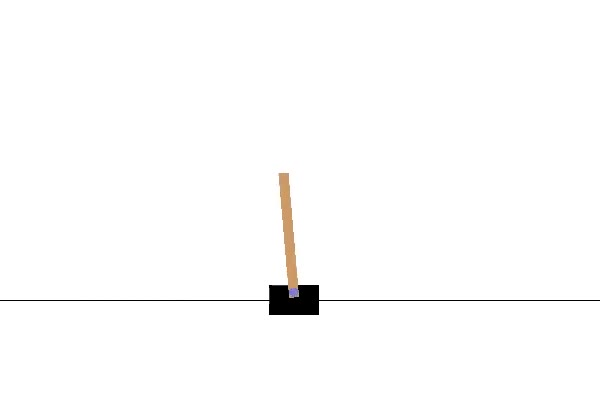
\includegraphics[width=0.5\textwidth]{cartpole-v0.jpg}
\caption{The CartPole environment \cite{gym2019cartpole}}
\label{fig:cartpole}
\end{figure}

As mentioned in Section \label{sec:arma}, clips are annotated according to the ground truth reward function of the environment. There are several ways of implementing this function which all encode the same goal of keeping the pole upright; see Appendix \ref{appendix:a} for the function we use. This reward function is hidden from the agent; it receives only rewards from the reward model, which is trained on preferences according to the ground truth reward.

To evaluate the performance of agents, we use the ground truth reward function as in \cite{Christiano2017}. As with many RL environments provided by OpenAI Gym, there is a defined threshold above which the agent is considered to have ``solved'' the environment. Our performance metric is the number of preferences required for an agent to reach this threshold.

Figure \ref{fig:cartpole_curve} shows our first attempt to train agents using reward modelling in CartPole. As the reward model is trained on an increasing number of labels, the mean episode return of the agents tends to improve. For clarity, the plot shows only random acquisition and BALD, though we tried all four acquisition functions and found no significant differences. We replicate the finding in \cite{Christiano2017} that active learning does not significantly improve on random acquisition. Our hypotheses about the cause of this negative result will be tested in the following sections. For reference, the mean episode return achieved by a standard RL agent (which can solve CartPole perfectly); taking random actions (\textit{random policy}); and training on a randomly initialised reward model (\textit{random reward model}) are also shown.

We found that even in a task as simple as CartPole, the performance of agents trained via reward modelling has high variance and low stability. For instance, using rewards from a reward model trained on \textit{more} labels sometimes leads to lower mean episode return. The results in Figure \ref{fig:cartpole_curve} were averaged over 40 repeats, which was required to decrease standard error from its initial high value. This suggests that whilst reward modelling has been shown, in some sense, to ``work'', it is not a mature technology and requires much more development before it could be applied to more real-world tasks. High variance and low stability is also reported by \cite[p.~7]{Christiano2017}, but they do not address the issue in much depth. It is worth noting that deep RL in general suffers from these same problems \cite{rlblogpost}.

\begin{figure}[h]
	\centering
	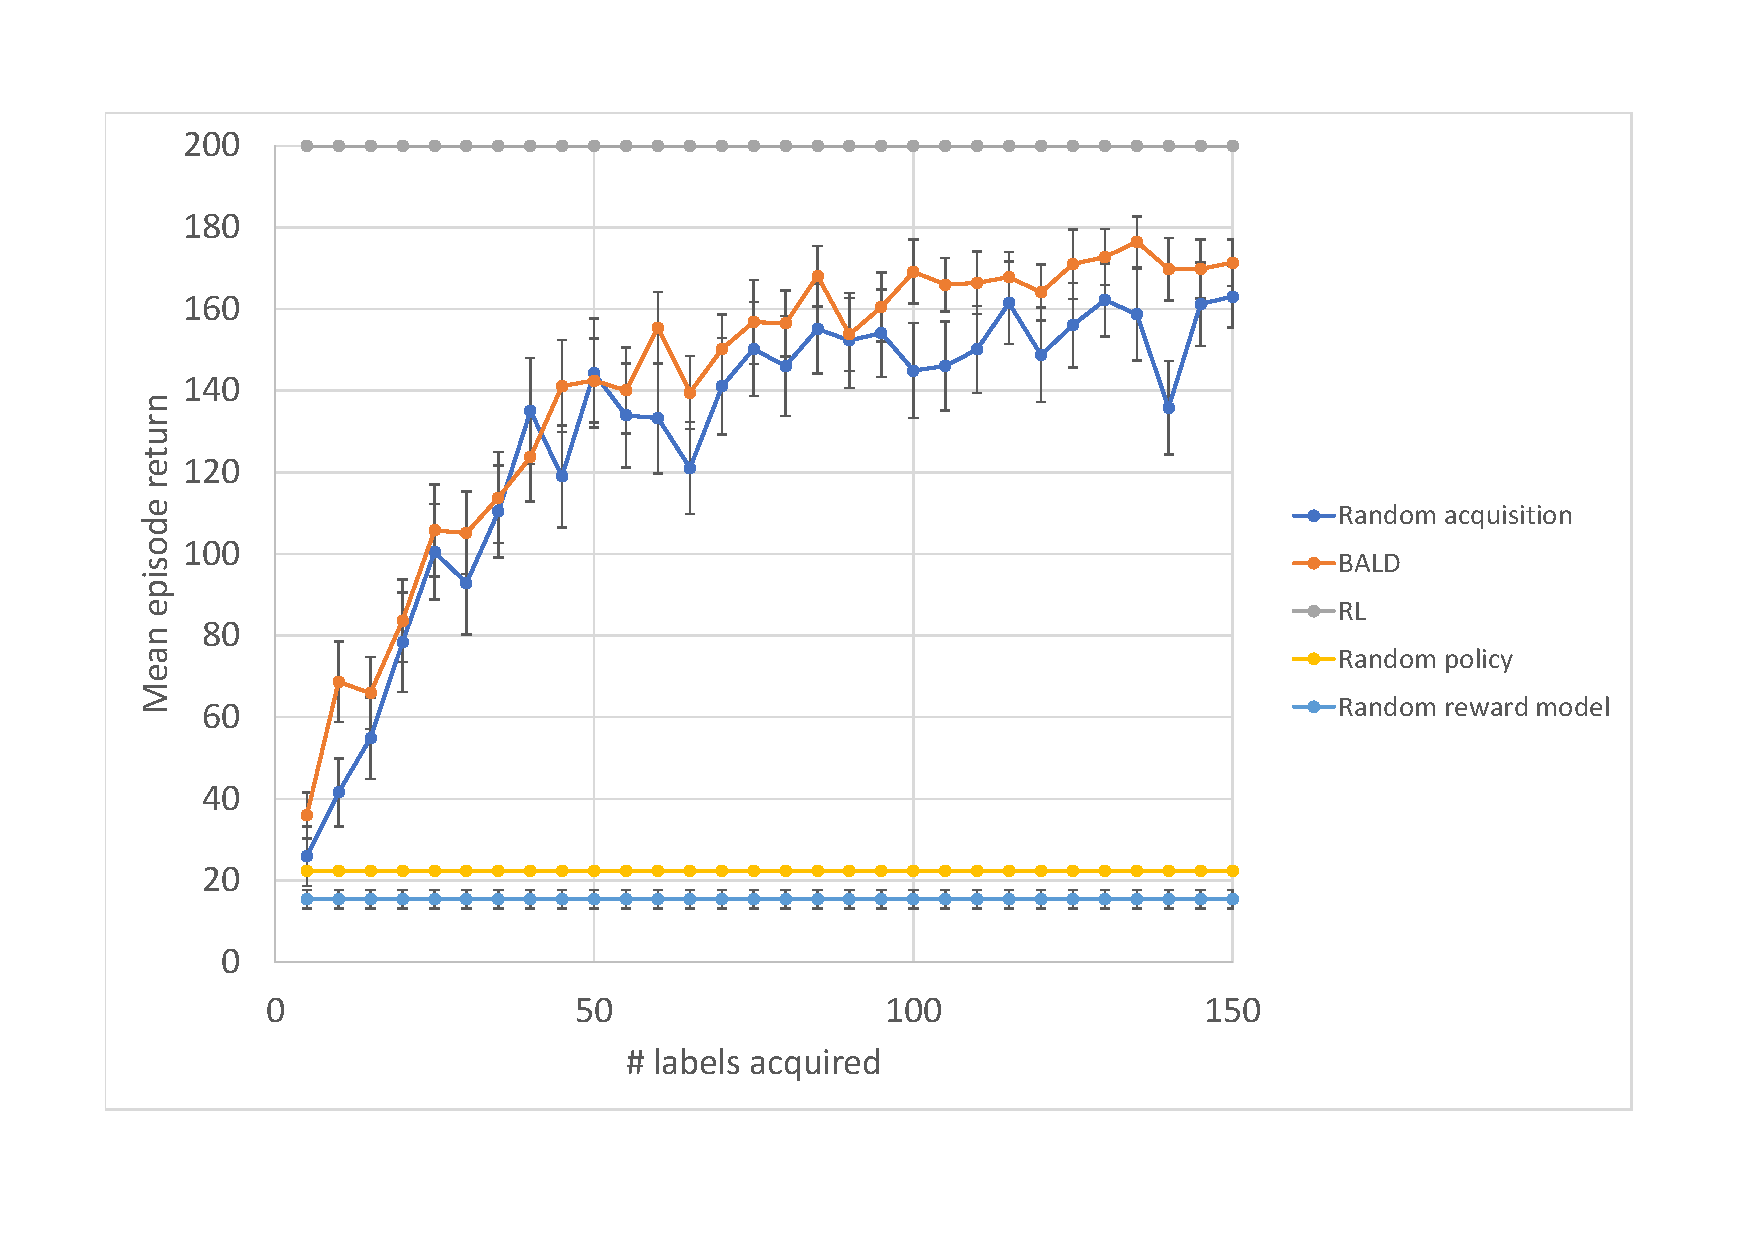
\includegraphics[width=\textwidth]{cartpole_curve}
	\caption{Mean episode return of agent trained via reward modelling using random acquisition and BALD. The performance of standard RL, a random policy, and an agent trained on a randomly initialised reward model are also shown. Results are averaged over 40 runs except for the random reward model condition which is averaged over 20. Error bars show standard error. Note that the performance of the agents trained via reward modelling is worse than those in the following sections due to less extensive hyperparameter tuning.}
	\label{fig:cartpole_curve}
\end{figure}

\section{Hypothesis 1: Reward model retraining}
Our first experiment tests the hypothesis that not retraining the reward model from scratch after every acquisition gives low quality uncertainty estimates. We run the training protocol given in Algorithm \ref{alg:arma} twice in the CartPole environment, changing whether the reward model is reinitialised in this manner. On each round, 5 preferences are acquired.

As shown in Figure \ref{fig:retrain}, we find that under both conditions, random acquisition and BALD show similar performance, but reward model retraining improves the performance of both. Therefore, whilst it is possible that the uncertainty estimates are harmed by not retraining, it is unclear how much of BALD's performance improvement is due to reward model retraining being better practice in general, because it gives equal weight to all the acquired data (the reason for which we see improvement in random acquisition, too).
\begin{figure}[h]
	\centering
	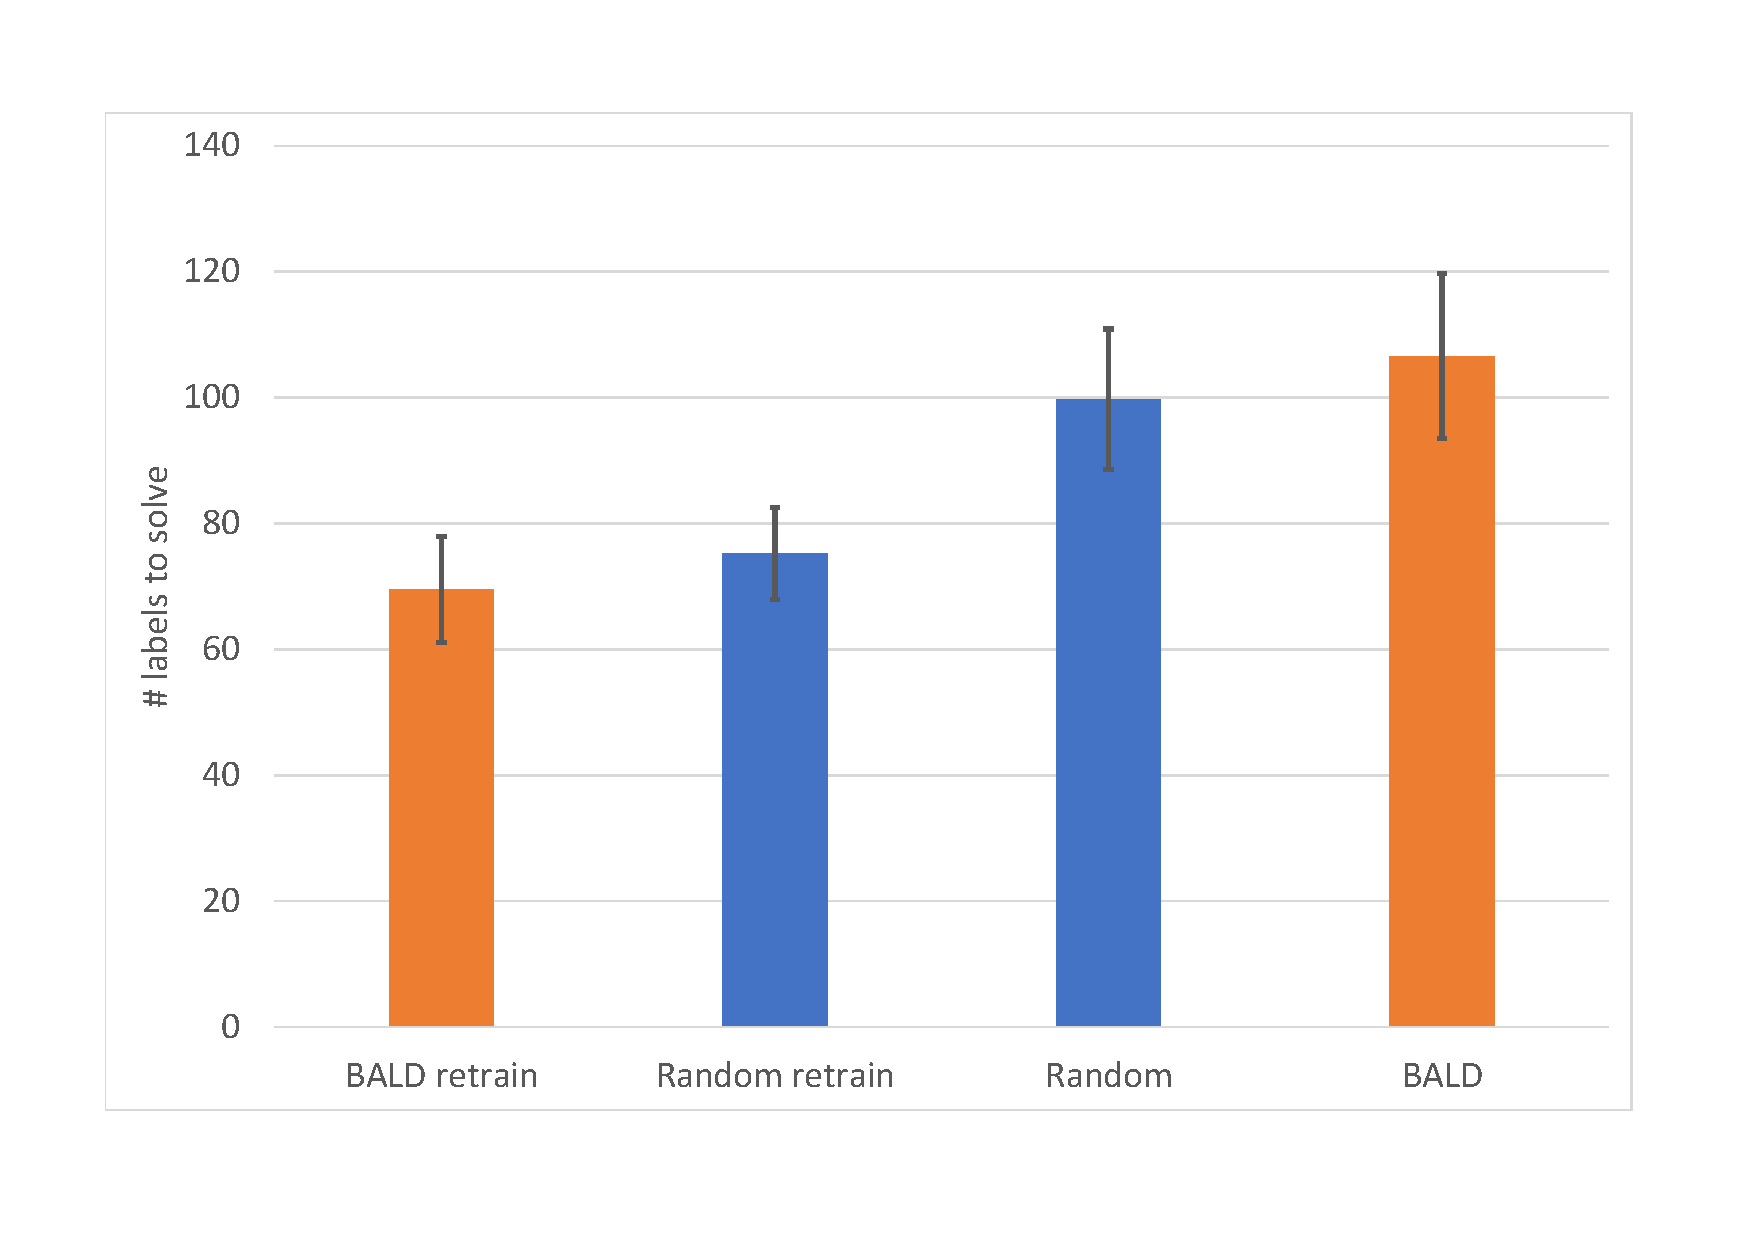
\includegraphics[width=0.75\textwidth]{reinit_rm}
	\caption{Number of labels required to solve CartPole by reward modelling with random acquisition and BALD, with and without retraining reward model after each acquisition. Results are averaged over 20 runs; error bars show standard error.}
	\label{fig:retrain}
\end{figure}

\section{Hypothesis 2: Acquisition size}
Next, we test the hypothesis that making acquisitions of size greater than 1 harms the performance of BALD-driven reward modelling. We run the training protocol in CartPole with acquisition size 10 and 1, retraining the reward model from scratch after each acquisition, and find that performance improves when acquisition size is reduced from 10 to 1, as per Figure \ref{fig:acq_size}. This indicates that when the acquisition size is too large, BALD acquires clip pairs that are individually informative, but are jointly less informative than the sum of their parts.
\begin{figure}[h]
	\centering
	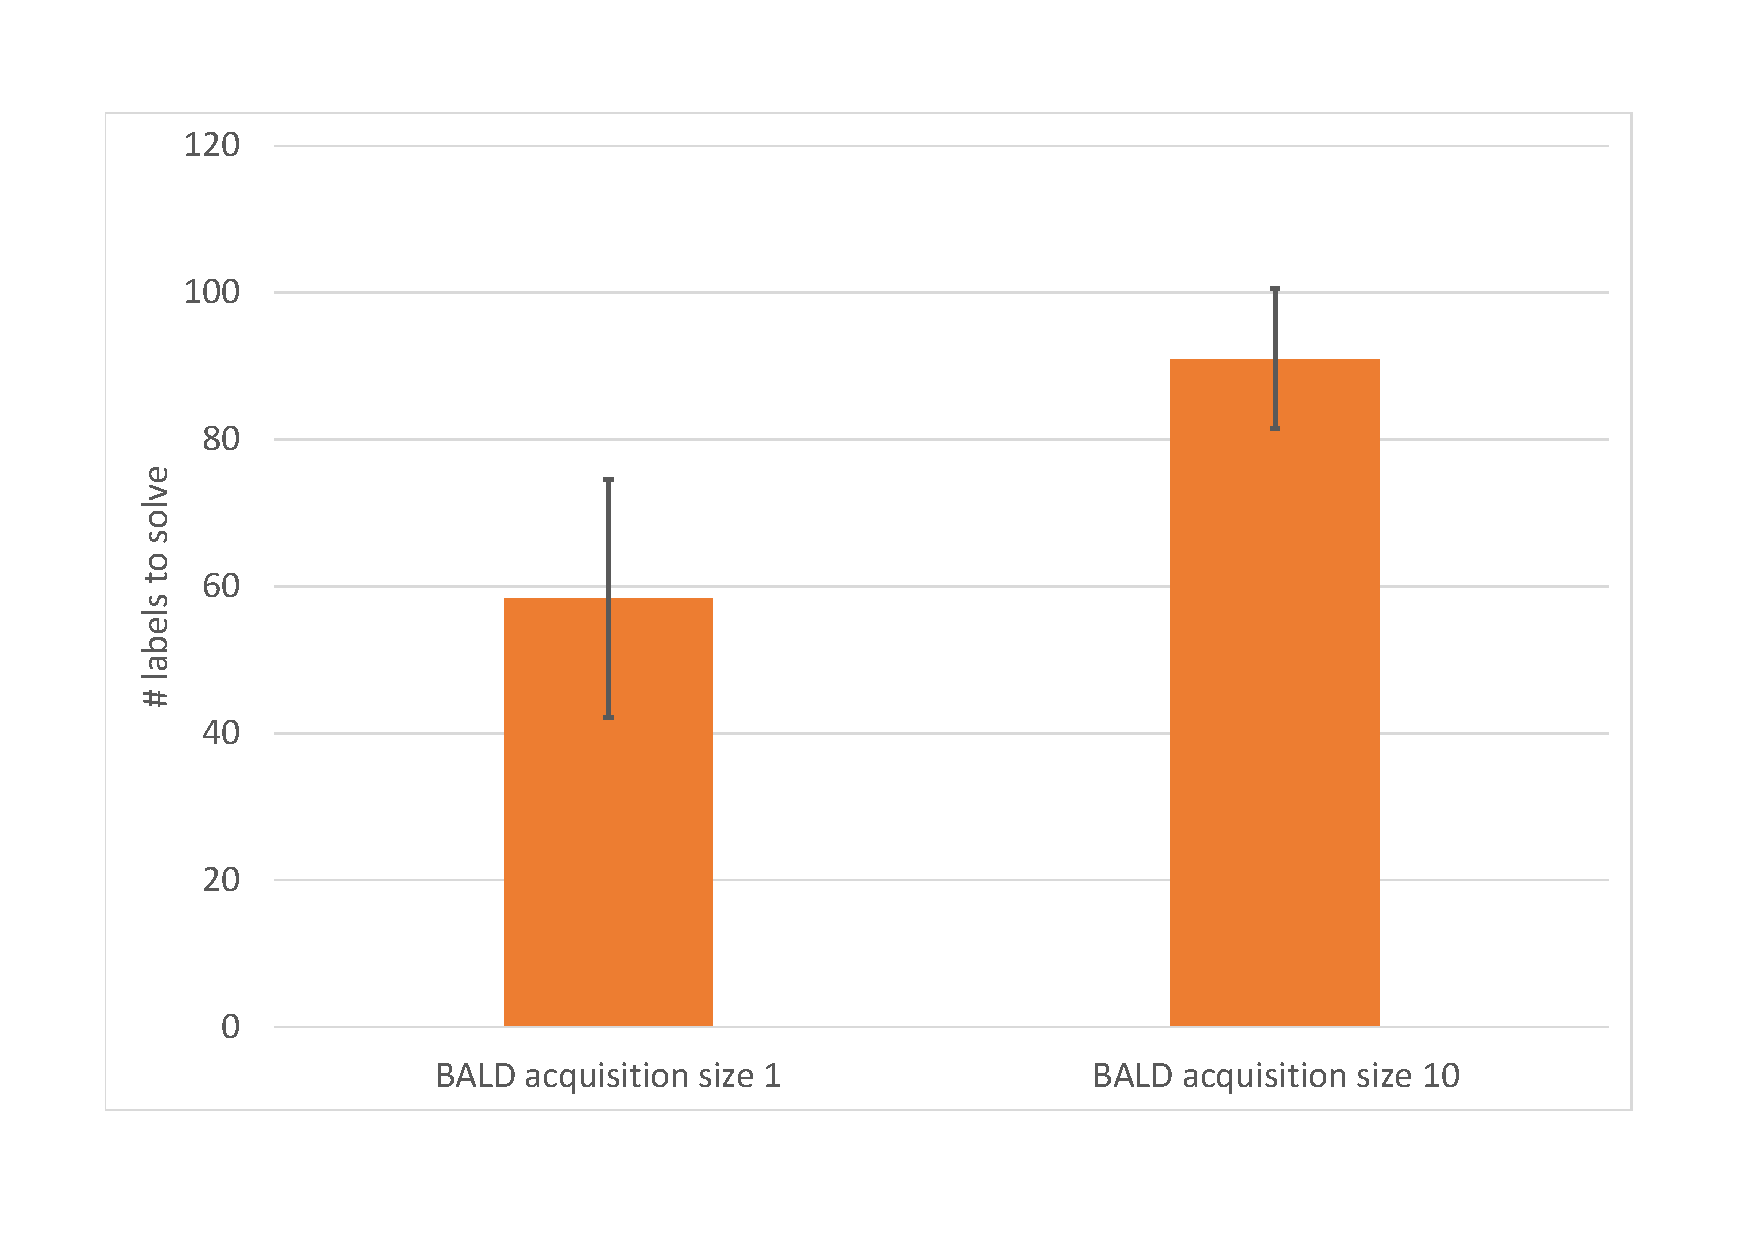
\includegraphics[width=0.75\textwidth]{acq_size}
	\caption{Number of labels required to solve CartPole by reward modelling with BALD, using acquisition sizes 1 and 10. Results are averaged over 20 repeats for acquisition size 10 and 6 repeats for acquisition size 1; error bars show standard error.}
	\label{fig:acq_size}
\end{figure}

\section{Hypotheses 3 and 4: Uncertainty estimate method and acquisition functions}
Having established that---in the CartPole environment---not retraining the reward model from scratch after every acquisition, and using large acquisition sizes harms the performance of active reward modelling, we retest all four acquisition functions with reward model retraining and acquisition size 1 compared to the random acquisition baseline. We also evaluate random acquisition using an ensemble of reward models, to ensure that any performance gains from active learning are not simply due ensembling. We also compare using MC-Dropout for estimating uncertainty with the ensemble approach taken so far.

Our results, summarised in Figure \ref{fig:cartpole_final}, show improved performance in general, but still no significant difference between random acquisition and active learning
\footnote{Note that BALD and random outperform their best results in the first two experiments because in between these experiments we performed extensive DQN hyperparameter tuning. Additionally, we found that not retraining the \textit{agent} from scratch on each round also impairs performance, as mentioned in Section \ref{sec:arma}. Being independent of the reward modelling aspect of the training protocol, such modifications affect all conditions equally and thus do not invalidate the results; they merely help to speed up experiments because agent performance performance is not harmed by having been trained (without subsequent reinitialisation) on a lower quality reward model.}.
This provides evidence against the hypothesis that the choice of acquisition function or uncertainty estimate method has a significant effect on the performance of active reward modelling. Contrary to the suggestion in \cite[p.~6]{Christiano2017}, merely changing these methods does not make active reward modelling improve on random acquisition, at least in the CartPole environment.

\begin{figure}[h]
	\centering
	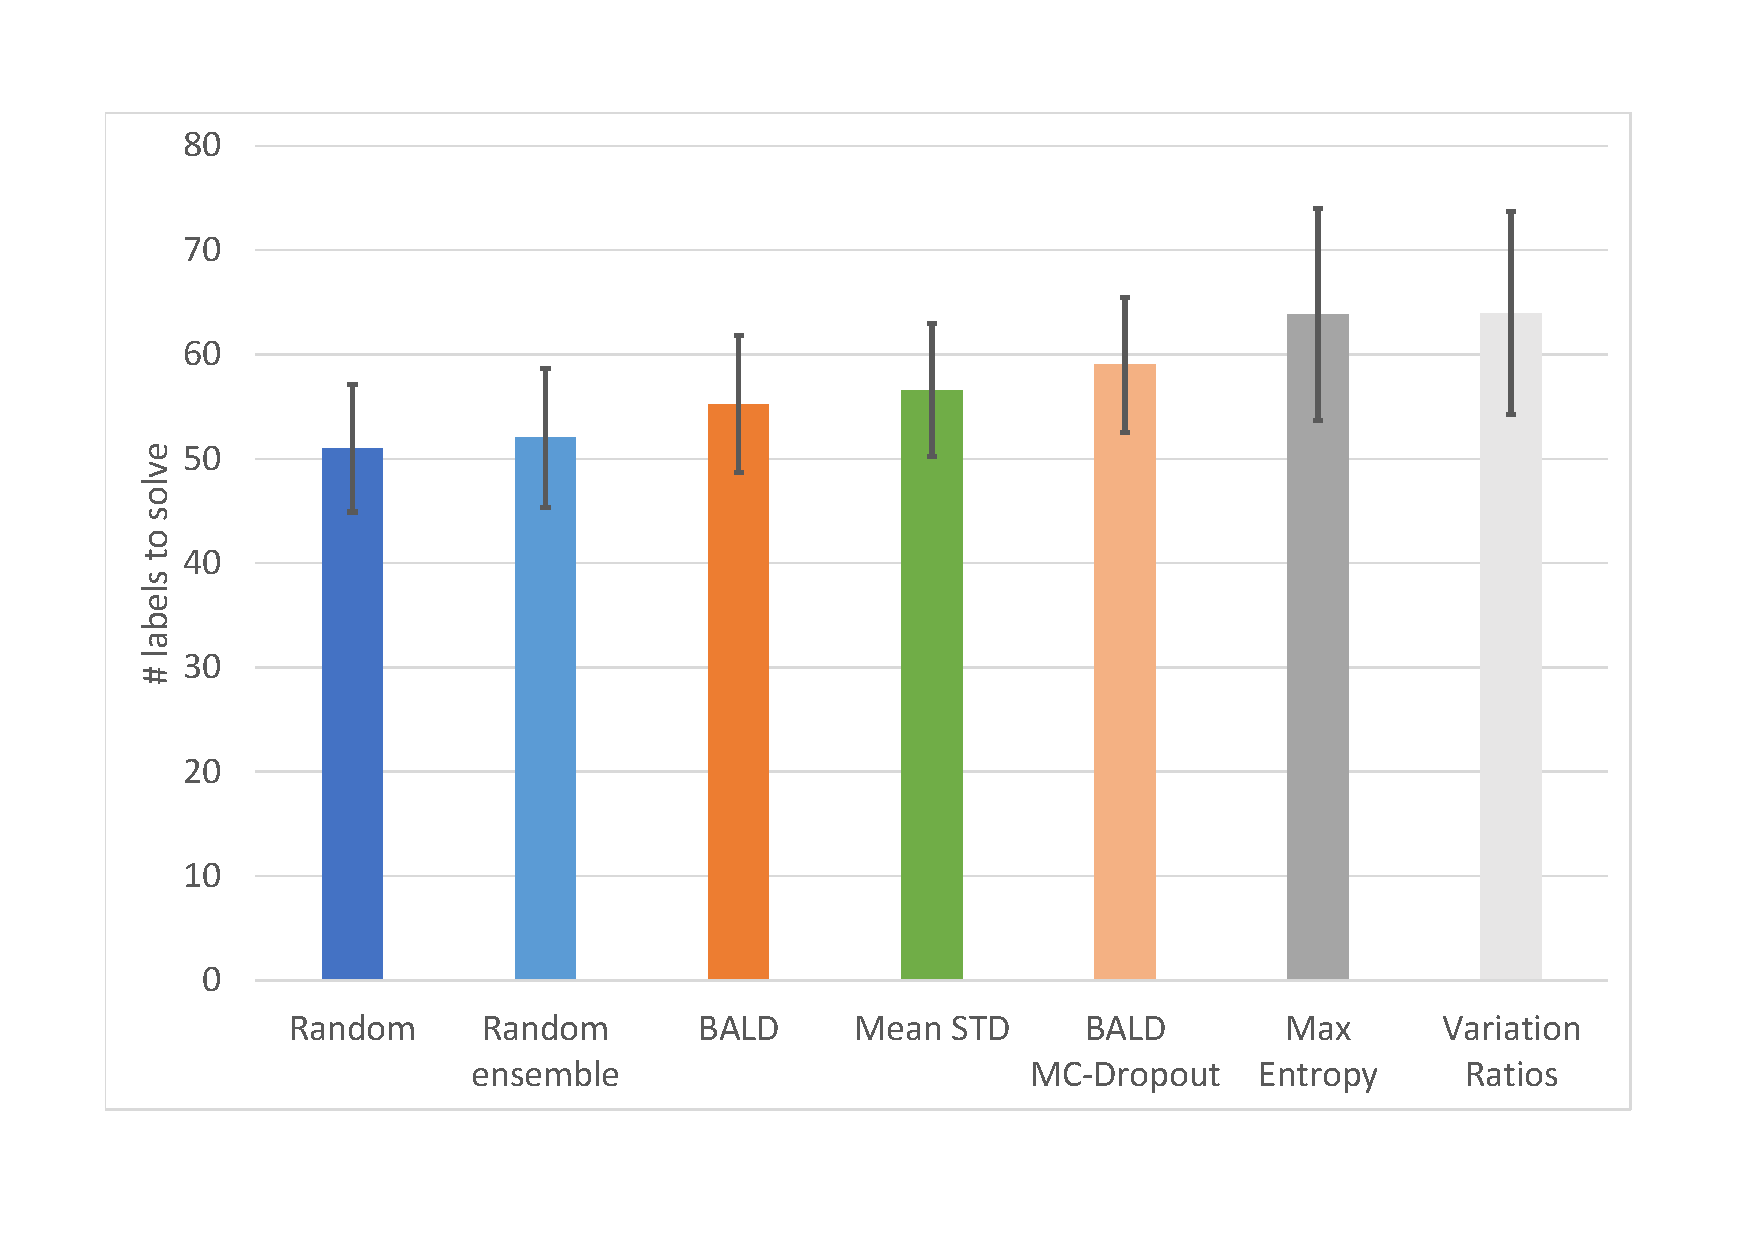
\includegraphics[width=\textwidth]{cartpole_final}
	\caption{Number of labels required to solve CartPole by reward modelling using various acquisition functions. The performance of using random acquisition with an ensemble of reward models, and BALD with uncertainty estimates from MC-Dropout with is also shown. Results are averaged over 20 repeats; error bars show standard error.}
	\label{fig:cartpole_final}
\end{figure}

In the experiments that follow, unless otherwise stated we continue to do reward model retraining and use acquisition size 1. Incorporating the latter modification by acquiring only 1 label per round, i.e. training the agent on the new reward model after every new acquisition, would make each experiment take a long time to run because agent training is a costly procedure. Therefore, we continue to acquire multiple labels per round, whilst using acquisition size 1. The procedure for doing so is shown in Algorithm \ref{alg:acq1}; this essentially replaces line \ref{line:sample_exp} to \ref{line:train_r} of the original training protocol given in Algorithm \ref{alg:arma}. The idea is simple: we repeatedly acquire 1 clip pair, query its label, reinitialise the reward model and train it to convergence, until $ m_i $ clip pairs are acquired and we proceed to agent training, and then onto the next round\footnote{Because reward model training also takes time, this modification will still slow down the training protocol. Future work could investigate whether a recent improvement on the BALD algorithm, called BatchBALD \cite{Kirsch2019a}, could successfully optimize this subroutine by removing the need to iteratively acquire single examples and retrain the model.}.
\begin{algorithm}
	\caption{Acquiring a batch of clip pairs with acquisition size 1.}
	\label{alg:acq1}
	\begin{algorithmic}[1]
		\State Sample $ 10m_i $ clip pairs from $ \expbuff $ \label{line:sample_exp2}
		\Repeat
		\State Acquire single clip pair that maximises $ a(.,.) $ \label{line:acq2}
		\State Request label on this clip pair (from the annotator) and add it to $ \annbuff $
		\State Reinitialise reward model $ \rp $
		\State Train $ \rp $ to convergence with the preferences in $ \annbuff $, by doing gradient descent on loss function \ref{eq:loss}
		\Until{$ m_i $ clip pairs have been acquired}
	\end{algorithmic}
\end{algorithm}

\section{Hypotheses 5 and 6: Quality of uncertainty estimates and ease of learning reward model}
Active reward modelling may be unable to outperform random acquisition due to poor quality uncertainty estimates, perhaps due to the reasons discussed in Section \ref{sec:failure2}, or an implementation bug. Furthermore, it may be that the CartPole task is simply too easy for active reward modelling to show improvement over random acquisition.

To test these hypotheses, we set up an experiment in which many duplicate clip pairs are added to the pool dataset. Essentially, this adds redundancy to the pool: once one of the duplicated clip pairs is acquired, no further information is gained about the annotator's latent reward function by acquiring exact copies of it.

More precisely, our experimental setup is to run the training protocol with both random acquisition and BALD, acquiring 5 labels per round (using acquisition size 1), with the following modification: after sampling $ 10\times 5 = 50 $ clip pairs from the experience buffer $ \expbuff $ (line \ref{line:sample_exp2} in Algorithm \ref{alg:acq1}), we make $ 10 $ identical copies of one of the clip pairs. Now, this set of $ 100 $ clip pairs is used as the pool dataset over which the acquisition function is evaluated on line \ref{line:acq2}. We call this setup \textit{Repeated CartPole}\footnote{This experiment was inspired by the \textit{Repeated MNIST} setup in \cite{Kirsch2019a}, which makes a somewhat similar modification to test a different hypothesis.}.

Modifying the procedure in this way will impair the performance of random acquisition. In expectation, 2.5 of the 5 randomly sampled clip pairs will be exact duplicates, meaning that the reward model is trained on a poorer quality dataset due to the redundant acquisitions. However, the performance of BALD should be unimpaired, because after acquiring one of the duplicate clip pairs, the information gained by acquiring the same clip again is zero, so BALD should not reacquire the example, but instead pick 4 other clip pairs from the original set. If, on the other hand, BALD is giving poor quality uncertainty estimates, then it will erroneously acquire duplicate examples and so the performance of BALD will also be significantly impaired in Repeated CartPole.

As shown in Figure \ref{fig:cartpole_rep}, we find that BALD's performance is not significantly harmed, whilst random acquisition performs poorly\footnote{The performance of BALD and random acquisition in the standard CartPole are both substantially better than in previous experiments. Having noticed the high variance of repeated experiments, we began testing agent performance several times on each iteration of the training protocol, rather than just at the end of agent training (testing agent performance means measuring mean episode return of the current policy in greedy forms, i.e. without taking random actions some $ \epsilon $ fraction of the time, over a fixed number of episodes, typically 100). This follows the testing regime used in \cite{Mnih2015}. Since this change is independent of the reward modelling aspect of the training protocol, it does not invalidate our previous results.}. This provides evidence that poor quality uncertainty estimates are not a failure mode of BALD in this environment.

\begin{figure}[h]
	\centering
	\begin{subfigure}{.5\textwidth}
		\centering
		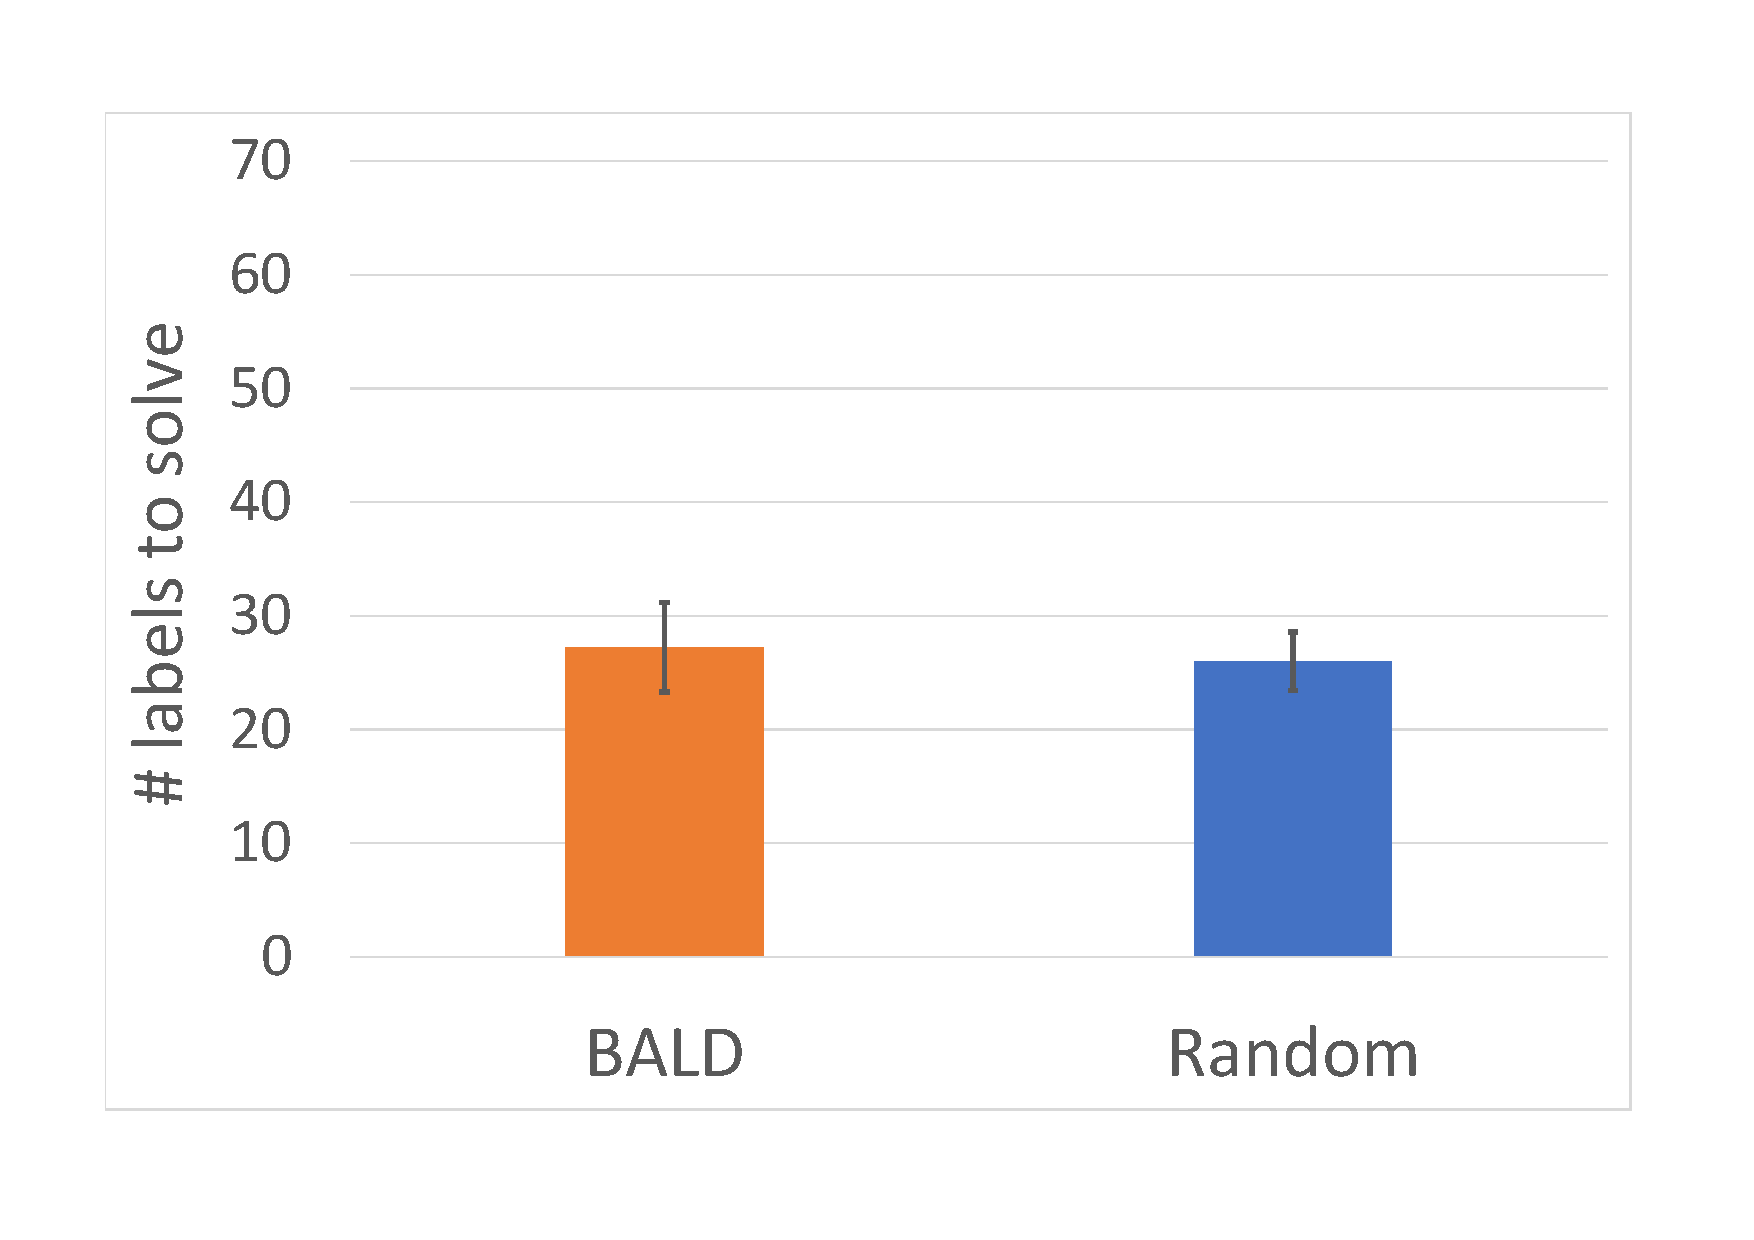
\includegraphics[width=\linewidth]{rand_bald_cartpole_final}
		\caption{Standard CartPole}
		\label{fig:sub1}
	\end{subfigure}%
	\begin{subfigure}{.5\textwidth}
		\centering
		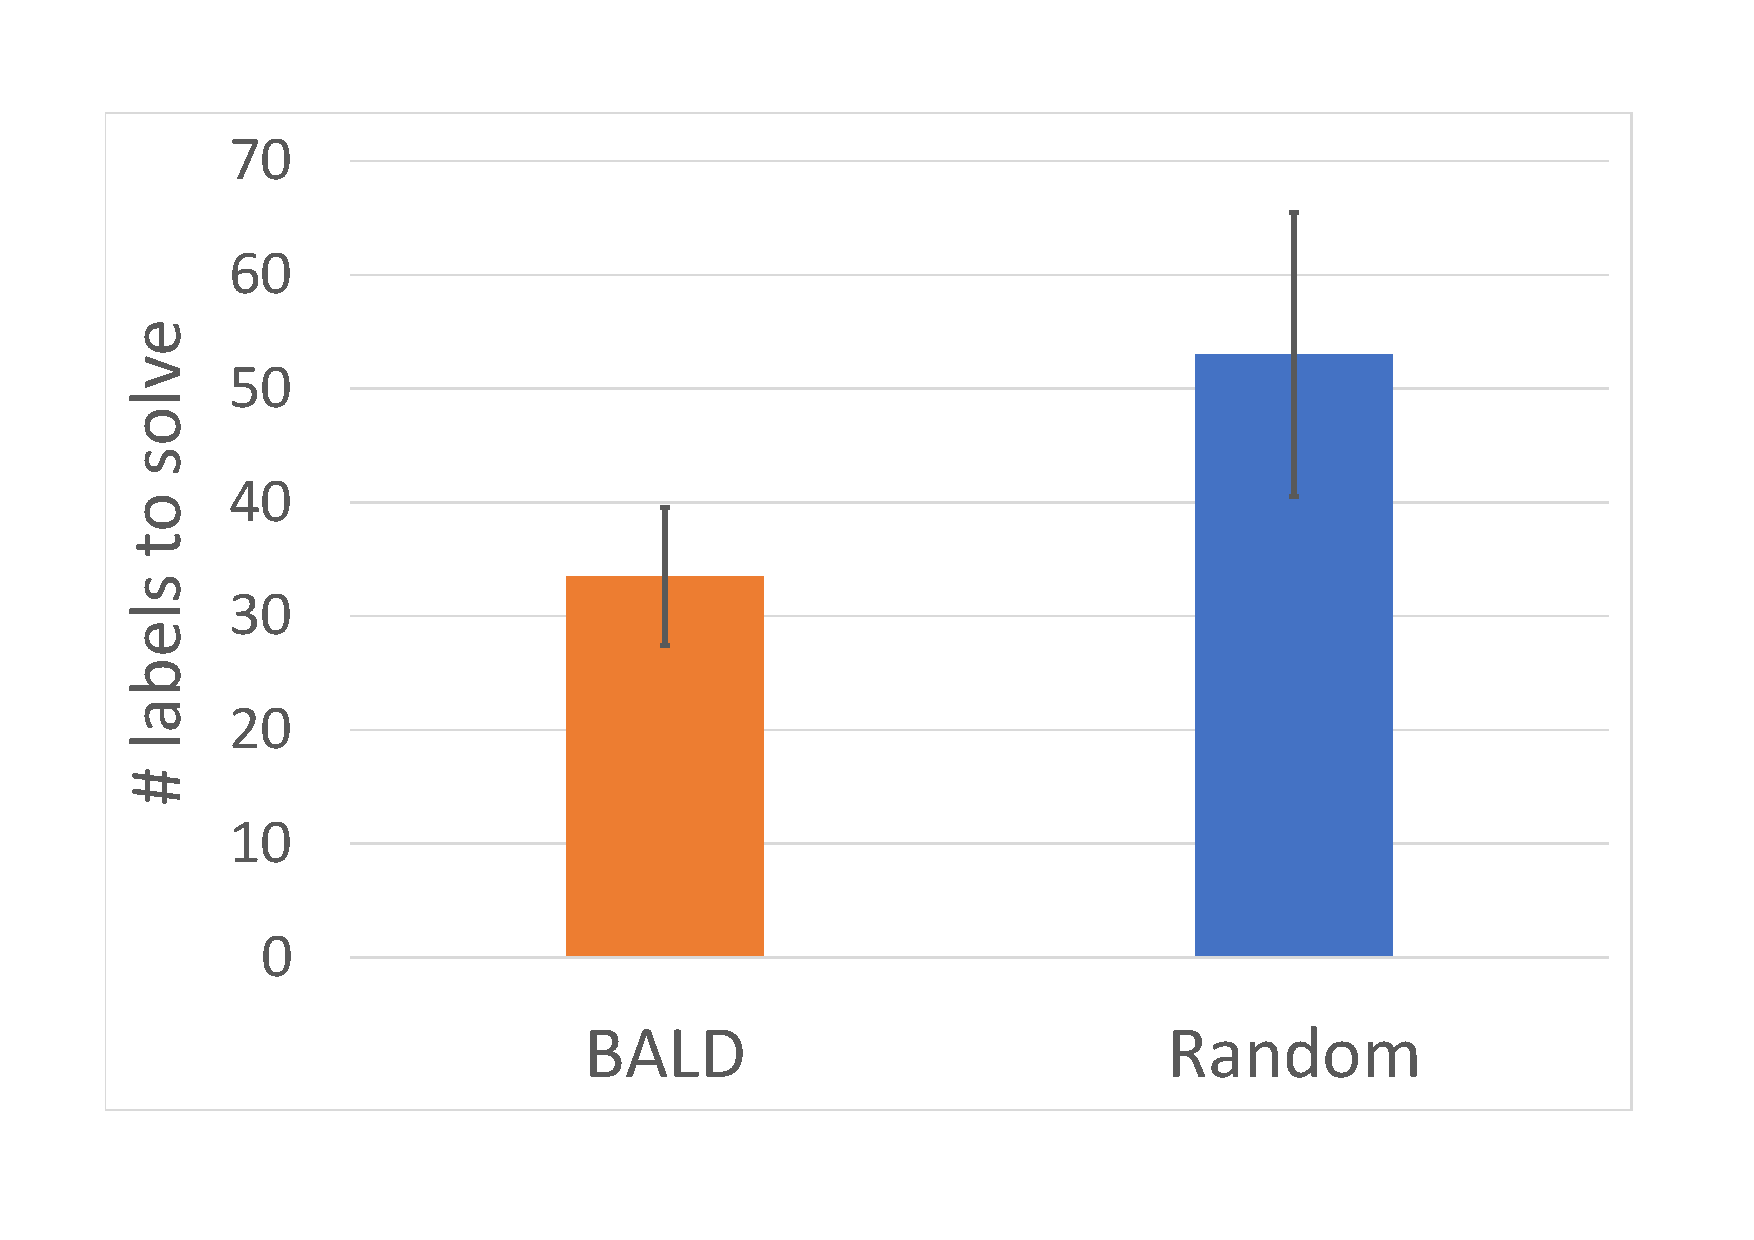
\includegraphics[width=\linewidth]{cartpole_rep}
		\caption{Repeated CartPole}
		\label{fig:sub2}
	\end{subfigure}
	\caption{Number of labels required to solve two variants of CartPole, using BALD and random acquisition functions for sampling clip pairs. Results are averaged over 20 repeats; error bars show standard error.}
	\label{fig:cartpole_rep}
\end{figure}

We gathered further evidence on the quality of BALD's uncertainty estimates by comparing the mutual information scores in Repeated CartPole with those in standard CartPole. Since there are many redundant examples in the pool dataset of Repeated CartPole, we expect BALD the average mutual information over this dataset to be higher than that in standard CartPole. However, as shown in Table \ref{table:2}, we find the opposite result. Whilst we would have liked to explore this further, it suggests that whilst BALD's uncertainty estimates are sufficient to outperform random acquisition in the Repeated CartPole setting, they are nonetheless far from perfect.

\begin{table}[]
\begin{tabular}{lllll}
	\cline{1-3}
	\multicolumn{1}{l|}{}                                     & CartPole     & Repeated CartPole &  &  \\ \cline{1-3}
	\multicolumn{1}{l|}{Average MI of BALD over pool dataset} & $ 0.06 \pm 0.01 $ & $  0.16 \pm 0.02 $      &  &  \\ \cline{1-3}
	&              &                   &  &  \\
	&              &                   &  & 
\end{tabular}
\label{table:2}
\caption{Mean mutual information over the pool dataset in CartPole and Repeated CartPole experiments, averaged over all acquisitions, with standard error from four repeat trials.}
\end{table}

One explanation of this result is that, as mentioned in Section \ref{sec:failure1}, BALD (and other acquisition functions) are known to give poor quality uncertainty estimates in the early stages of training. For instance, Figure 1 of \cite{Gal2017b} shows no significant difference between the performance of BALD and random acquisition prior to acquiring the $ 50^\text{th} $ example. Given that reward modelling can solve CartPole with around 30 labels, BALD's inability to outperform random acquisition in this setting would be consistent with this result.

To summarise the results so far, we have shown that in the CartPole environment, not reinitialising the reward model and using large acquisition sizes harms active reward modelling, and the former problem also harms non-active reward modelling. This provides evidence for hypotheses 1 and 2 being failure modes of active learning in this environment. With these changes, however, active reward modelling still cannot outperform random acquisition, so these are not the only failure modes. We then provided evidence against hypotheses 3 and 4 by comparing four common acquisition functions and two uncertainty estimates methods and finding that no combination improves on random acquisition. Finally, the Repeated CartPole experiment suggests that the uncertainty estimates are of questionable quality in CartPole, yet they are not so poor as to render BALD unable to distinguish duplicate clip pairs.

\section{Gridworld experiments}
A gridworld is a simple two-dimensional environment of size 4x4, containing an agent (blue), one goal cell (green) and an optional lava cell (red). On each time step, the agent receives an observation of the environment, which is an RGB pixel value for each cell, and takes one of four actions (up, down, left or right). The environment gives rewards of $ +1 $ for reaching the goal, $ -1 $ for moving onto the lava, and $ 0 $ otherwise. Episodes terminate when the goal or lava is reached, or when 50 time steps have passed. An example state of the environment is shown in Figure \ref{fig:grid}. This is similar to the environment used in \cite{kenton2019generalizing}. We define solving this environment as getting a mean episode return of greater than $ 0.95 $ across 100 episodes, equivalent to reaching the goal in 95 of 100 episodes.

\begin{figure}[h]
	\centering
	\begin{subfigure}{.3\textwidth}
		\centering
		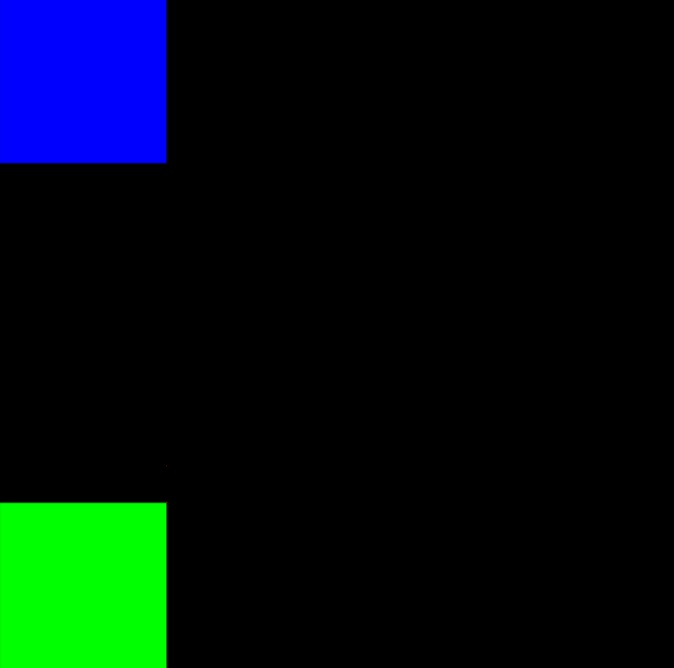
\includegraphics[width=\linewidth]{grid2}
		\caption{Gridworld with one goal cell.}
		\label{fig:grida}
	\end{subfigure}\hspace{.1\textwidth}
	\begin{subfigure}{.3\textwidth}
		\centering
		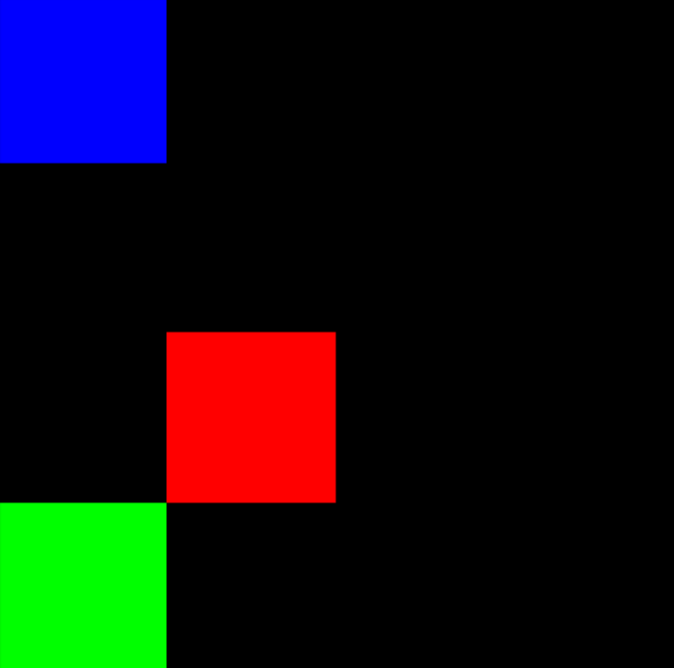
\includegraphics[width=\linewidth]{grid}
		\caption{Gridworld with one goal and one lava cell.}
		\label{fig:gridb}
	\end{subfigure}
	\caption{Two examples of possible gridworld environments. The blue, green and red cells are the agent, goal and lava, respectively.}
	\label{fig:grid}
\end{figure}

The simplest configuration of this gridworld has no lava cell and a goal cell with a fixed location. As a sanity check, we use this simplest configuration to try to replicate the finding that in simple tasks and environments, active reward modelling is unable to outperform random acquisition. Specifically, we fix the goal location to be in the bottom left corner, and the agent starting location to be in the top left corner, corresponding to Figure \ref{fig:grida}. By a quick simulation, we found that $ 17\% $ of the clips\footnote{We use clip length 10 here, rather than 25. TODO push all such details to the appendix.} generated by an agent taking random actions in this environment have total reward $ +1 $. This should mean that a decent proportion of the clip pairs acquired at random will contain information about synthetic annotator's preferences and so non-active reward modelling should be able to solve the environment with very few acquisitions, whilst BALD should suffer from poor quality uncertainty estimates, having only been trained on a small number of examples. Indeed, as seen in Figure \ref{fig:grid_simple} the results affirmed this.
%(As well as reward modelling using BALD and random acquisition, we evaluate agents that (i) do standard RL on the ground truth reward, (ii) take random actions and (iii) get reward from a random reward model.)

\begin{figure}[h]
	\centering
	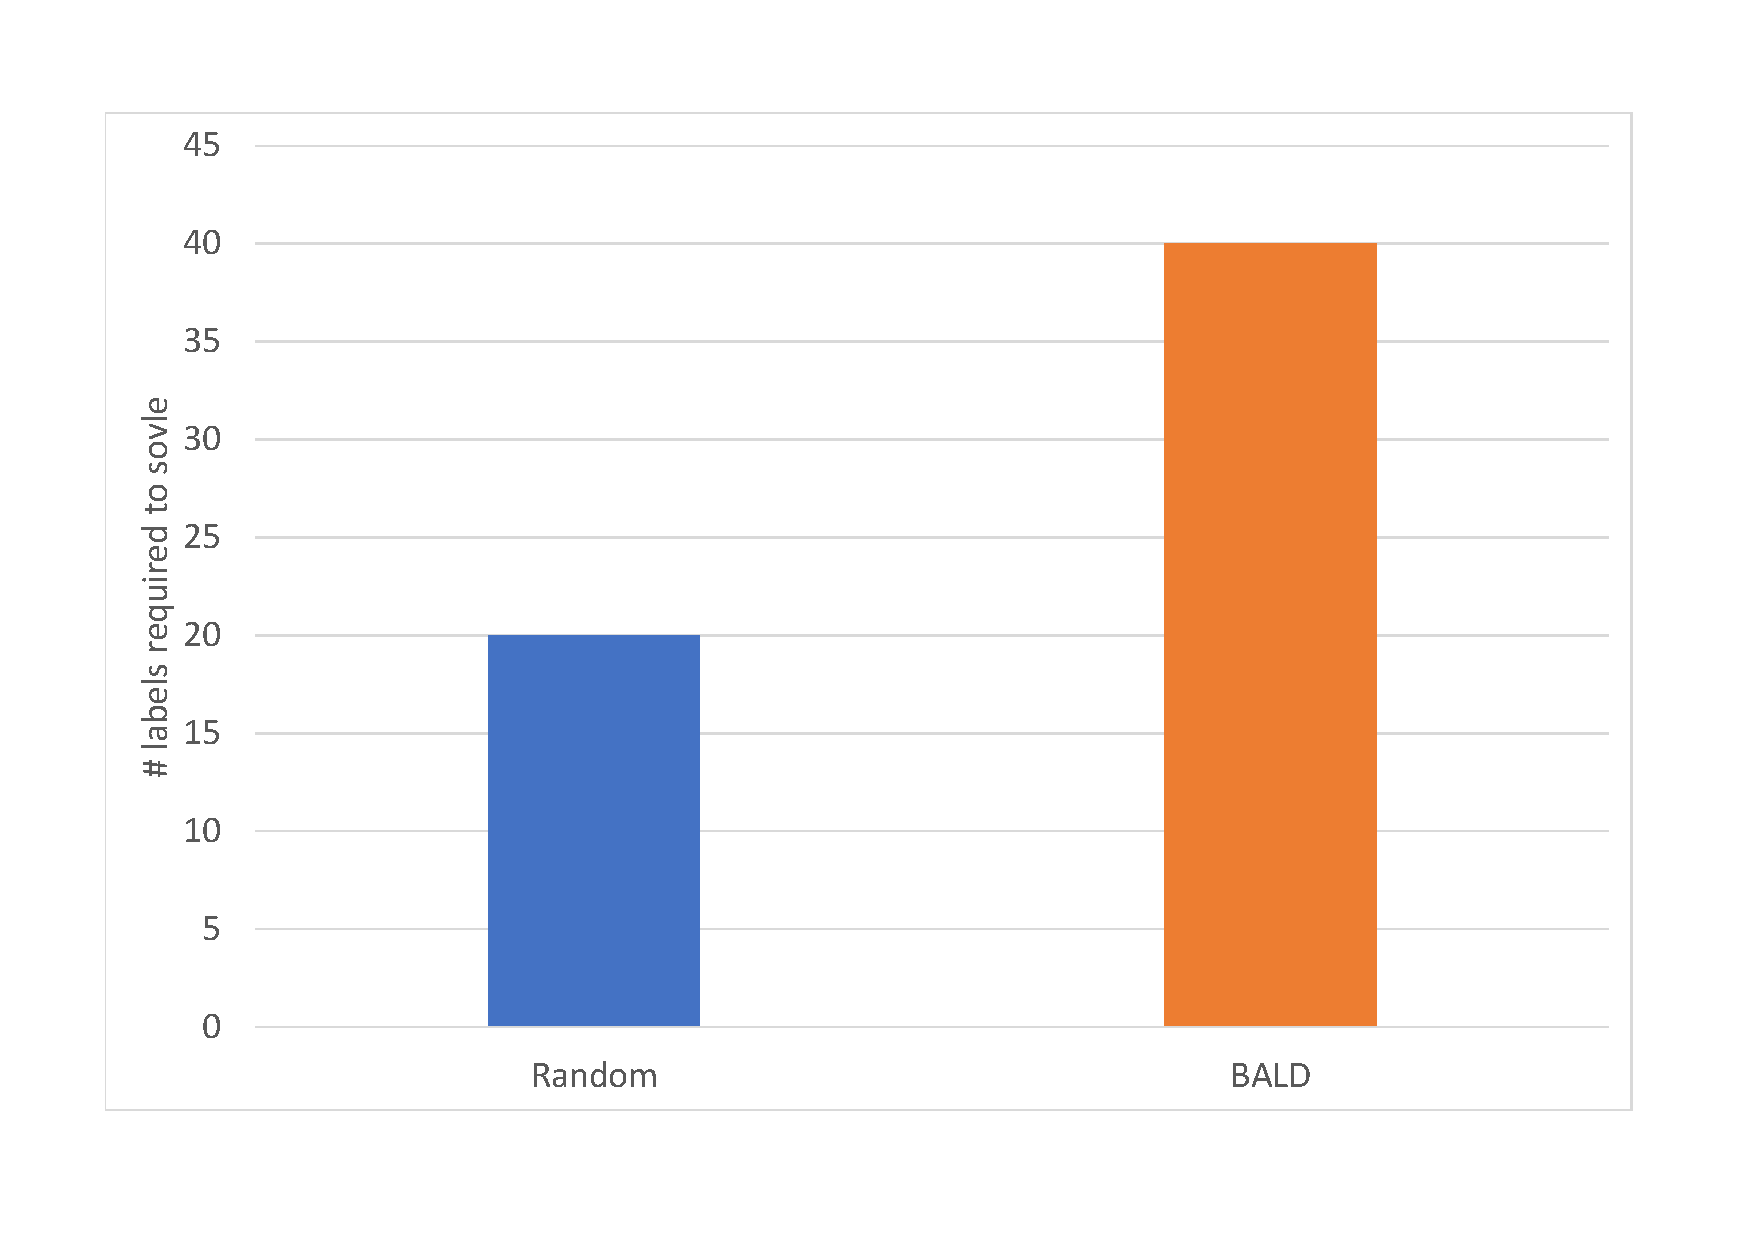
\includegraphics[width=\textwidth]{grid_simple}
	\caption{Number of labels required to solve the gridworld shown in Figure \ref{fig:grida} via reward modelling using BALD and random acquisition. Results shown are only one run.}
	\label{fig:grid_simple}
\end{figure}

\section{Uncertainty estimate quality in the gridworld environment}
Our results about the quality of uncertainty estimates in active reward modelling were inconclusive, in the sense that we were unable to tell whether the estimates were of questionable quality because the number of training examples was so small, or for some more fundamental reason. Our next gridworld is more complex, meaning that more labels are required in order to learn the annotator's reward function. Specifically, we introduce a lava cell, also with a fixed position, placing it close to the goal cell, as shown in Figure \ref{fig:gridb}. By a simulation, we found that around $ 95\% $ of clips sampled from the trajectories of a random policy have zero return, around $ 1\% $ have return greater than or equal to $ +1 $, and around $ 4\% $ have return less than or equal to $ -1 $. Because of the infrequency of clips with positive return, random sampling will collect few such clips, and therefore non-active reward modelling will struggle to learn the annotator's reward function. However, since such clips contain vital information, active reward modelling should acquire these clips. If it does not, then we should be sceptical about the quality of the uncertainty estimates.
%TODO mention clip length 1. Appendix?

\begin{figure}[h]
	\centering
	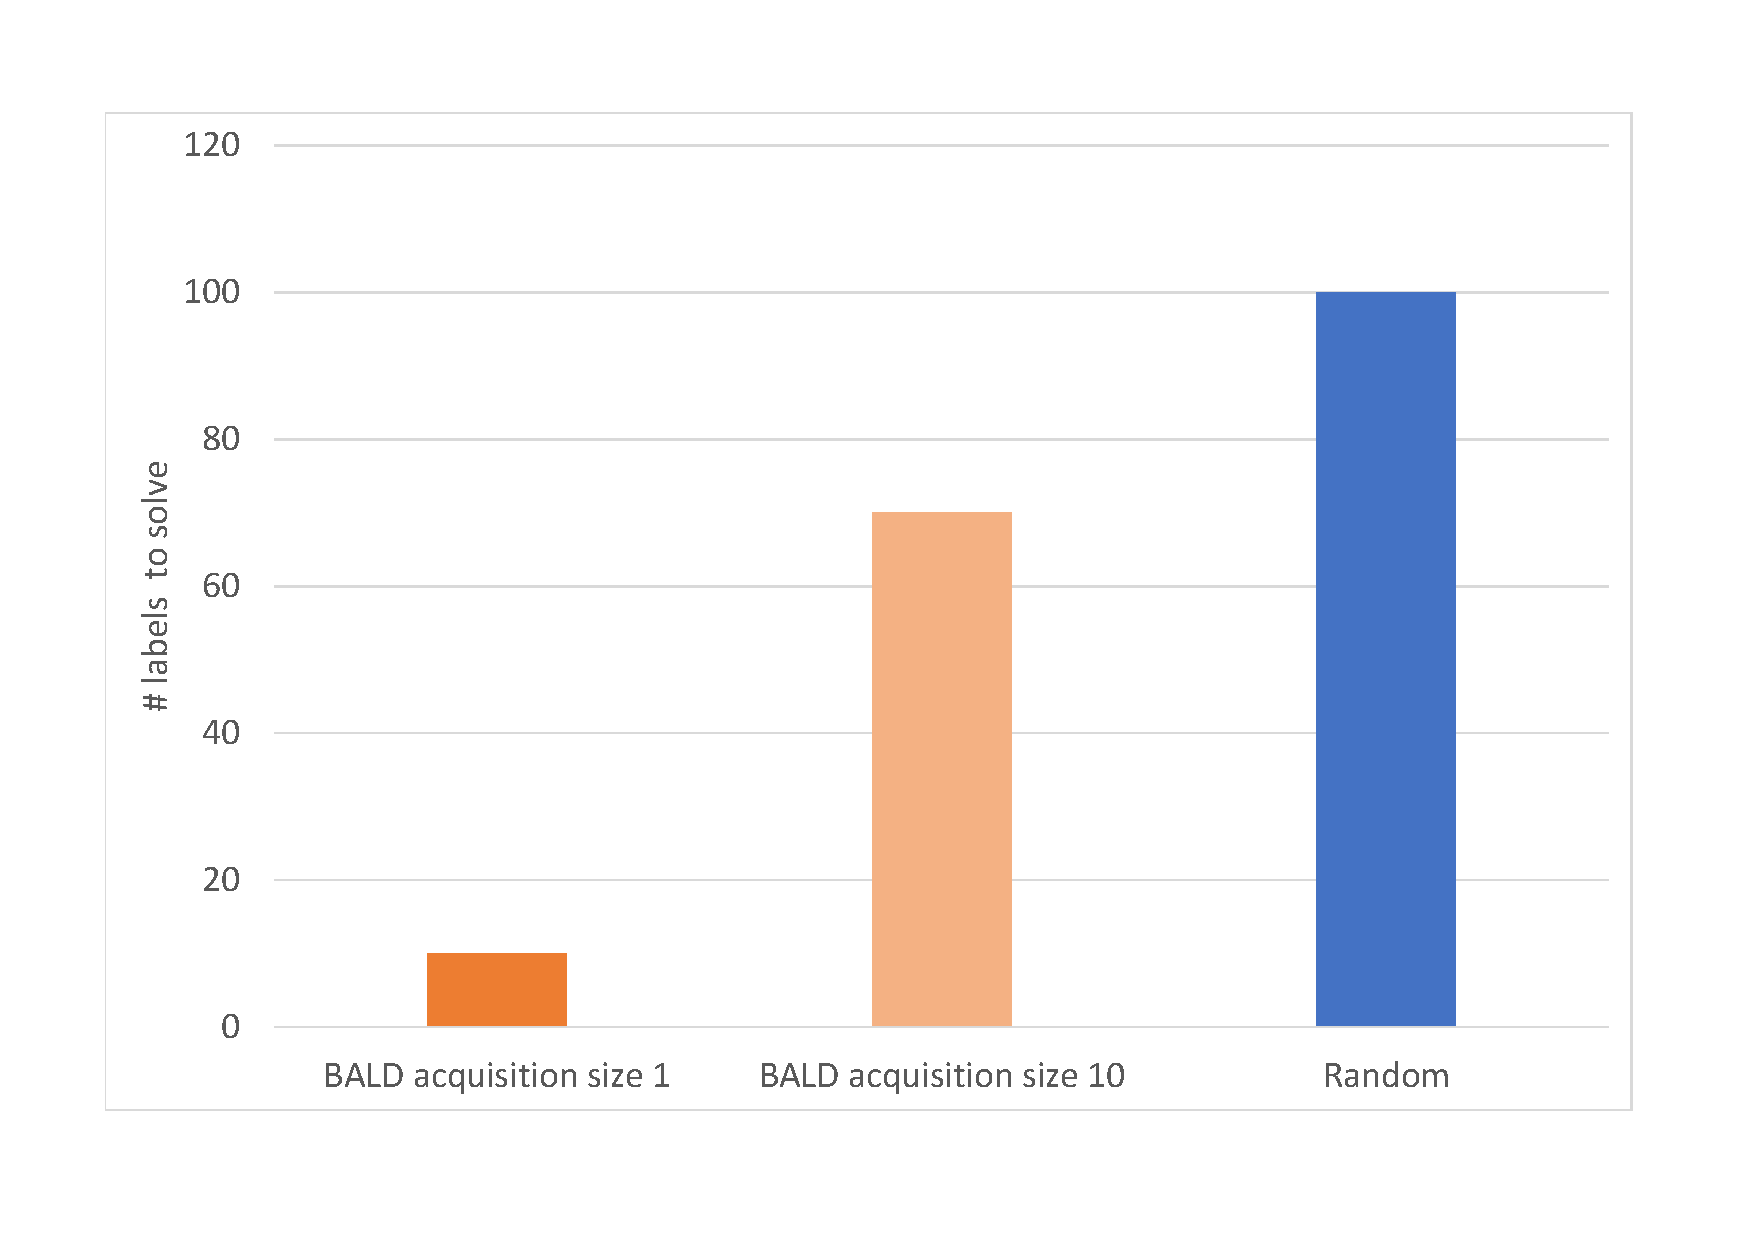
\includegraphics[width=\textwidth]{grid_medium}
	\caption{Number of labels required to solve the gridworld shown in Figure \ref{fig:gridb} via reward modelling using random acquisition, and BALD with acquisition sizes 1 and 10. Only one random seed is shown.}
	\label{fig:grid_medium}
\end{figure}

As shown in Figure \ref{fig:grid_medium}, the results provides good evidence that the uncertainty estimates in active reward modelling are of good enough quality to outperform random acquisition in this more complicated environment. We also evaluate BALD using acquisition size 10, and replicate the finding of Section \ref{sec:acq_size} this hurts the performance of BALD.
%TODO if time, add information about the acquisition profiles of BALD v random. BALD is seen to pick the rarer clips.

\section{Hypothesis 7: Active reward modelling exploration issues}
Finally, we shift our attention to the hypothesis that in even more difficult tasks, too few trajectories generated by the agent are informative, meaning that the pool dataset rarely contains informative clip pairs, and active learning is unable to acquire them. This failure mode applies to random acquisition as much as it does to active reward modelling, so we expect to see both methods failing in such environments.

The setup is to make a small modification to the previous setting: using a clip length of 10, instead of 1. As noted in \cite[p.~10]{Christiano2017}, using shorter clips is more helpful \textit{per frame}, but less helpful \textit{per clip}. This is because longer clips introduce some kind of ``credit assignment'' problem. A reward model trained a particular pair of long clips has no way to infer which actions in the clip were preferred by the annotator; only after receiving multiple similar clips can it infer, on the level of granularity of actions, what the annotator's preferences are. However, if the annotator desires to align an agent to take particular long sequences of actions, using long clips is imperative.

In our small gridworld, this is not the case. We set up the annotator's hidden reward function to give sparse rewards of $ +1 $ for reaching a goal cell and $-1$ for moving onto a lava cell, meaning that clips of length 1 are relatively more helpful than clips of length 10. Therefore, using longer clips should make the reward modelling task more difficult.

We evaluate the performance of using BALD and Mean STD to drive active reward modelling, against random acquisition, both using and not using an ensemble of reward models. We find that...
%TODO say a thing about doubly hard exploration
% also that the reward model test loss is converged so we are stuck with this behaviour.

\begin{figure}[h]
	\centering
	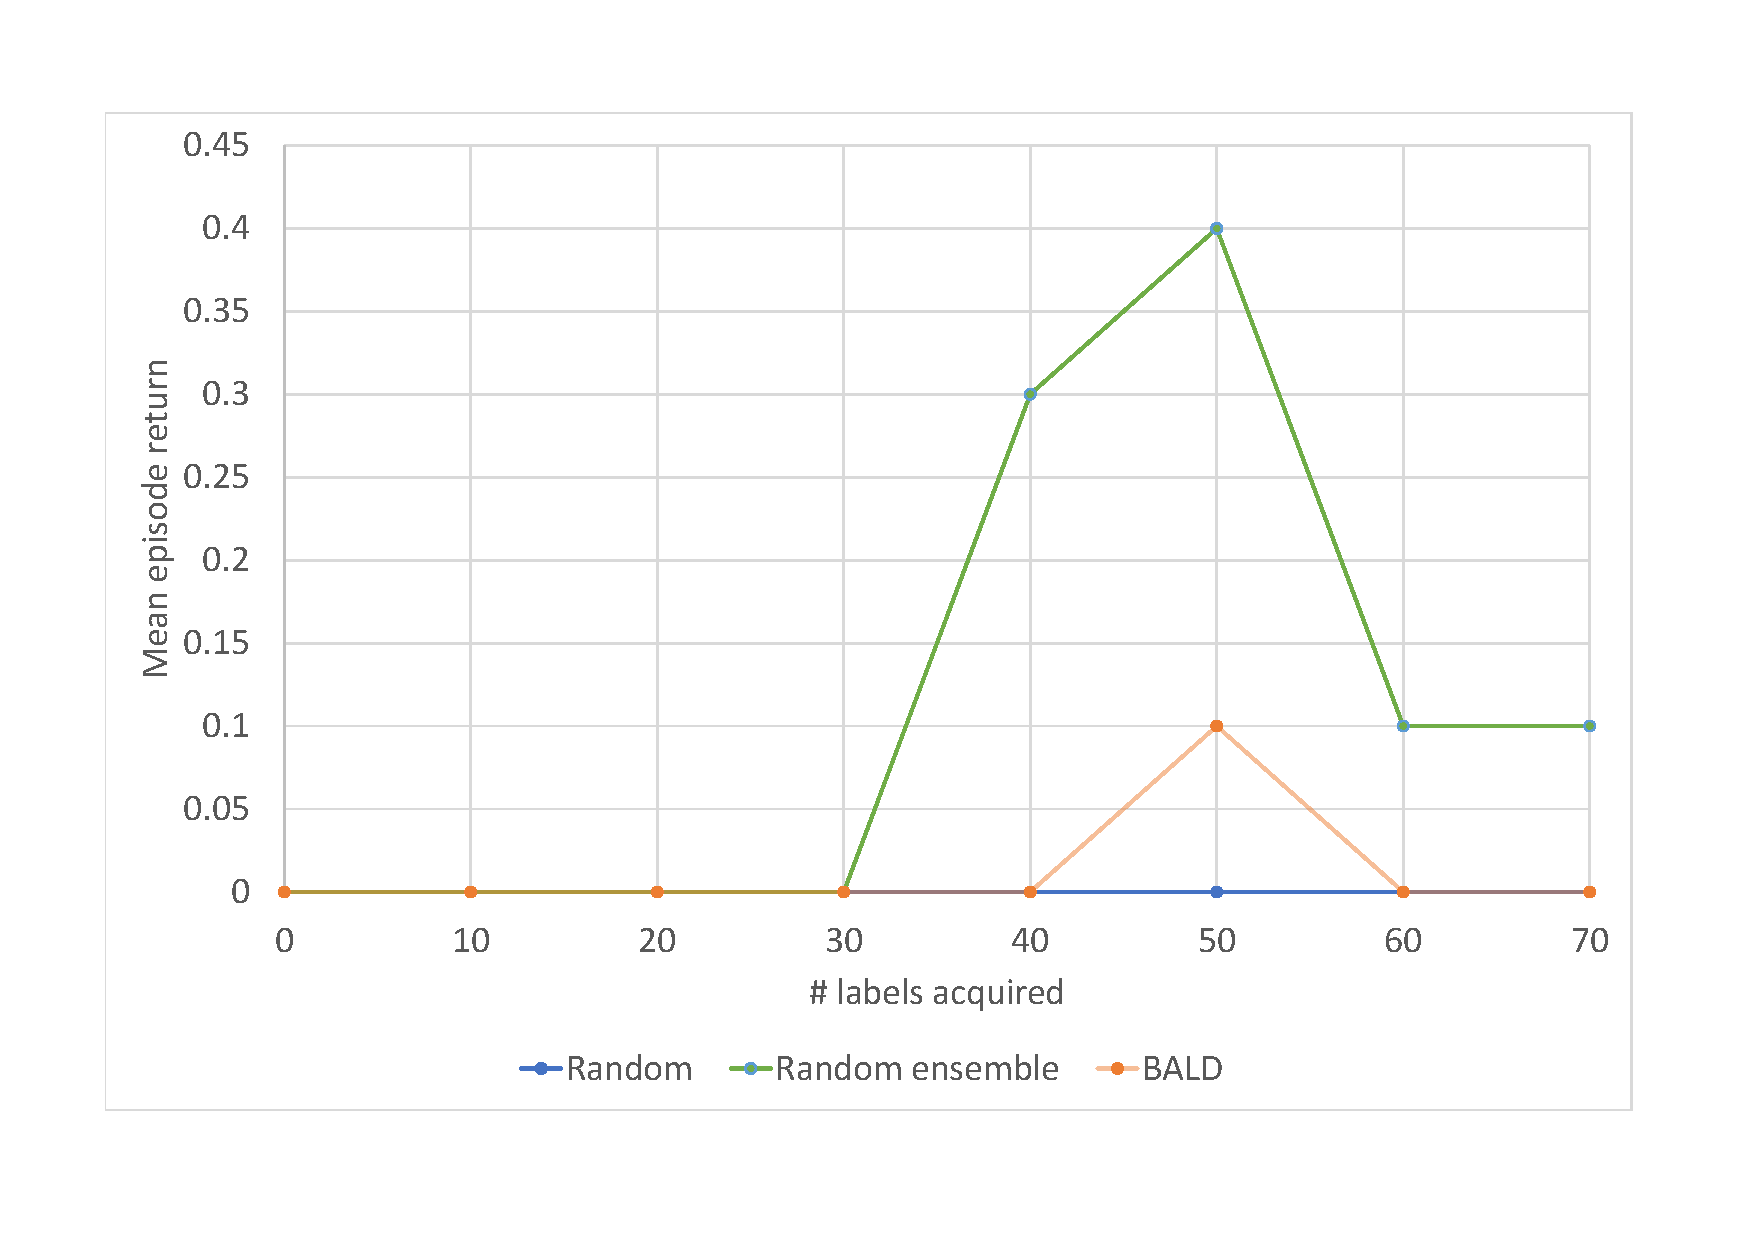
\includegraphics[width=\textwidth]{grid_hard}
	\caption{ Only one random seed is shown.}
	\label{fig:grid_hard}
\end{figure}



%The effect varying clip length is studied by \cite{Christiano2017}, who find that in simulated robotics tasks, using shorter clip length significantly impairs performance. 
%However, in this environment, the synthetic annotator prefers 

\chapter{Conclusions}
\section{Summary}
\section{Future Work}
\section{Relation to Material Studied on the MSc Course}
\section{Critical Evaluation}
% critical assessment of the work that has been done and the process of doing it
% perhaps include subsections for approaches that were tried and did not work; and personal development
\subsection{Personal Development}
Not to seek to make the thing work, but to wonder, why? To notice confusion rather than running from it. 'Acrobot shouldn't solve in one label'. Led to us finding it was a bad environment for testing reward modelling.
Random acquisition with ensemble underperforming random without ensemble early in training -> realised that not implementing per-component normalisation of reward models; not normalising at training time correctly. (Well, in fact this was a case of running from this confusion for ages, before finally---and begrudgingly---facing up to it. In some sense this was a key learning point; feeling that noticing confusion pays off in the long run.)
Ignoring occasional NaNs was another example. When I finally debugged it rationally, I found that normalising observations greatly improves reward model performance.





% acknowledgements

\bibliographystyle{apalike}
\bibliography{library,additional}

\appendix
\appendixpage
\noappendicestocpagenum
\addappheadtotoc
\chapter{Appendix A} \label{appendix:a}
\section{CartPole Experimental Details}
\subsection{Ground truth reward function}
OpenAI Gym implementation of CartPole gives $ +1 $ reward on every time step. Since we follow the approach taken in \cite{Christiano2017} where all clip pairs are of equal length, using this reward for the synthetic evaluation of clips would give the same total reward to every clip. Therefore, we instead use the reward function given in  \cite[p.~59]{Sutton2018}: $ 0 $ on every time step, except for failure steps---when the cart moves more than $ 2.4 $ units from the centre or the pole falls to more than $ 15 $ degrees from vertical---for which $ -1 $ is given. Note, however, that we use the OpenAI Gym reward for testing agent performance, because there is a defined threshold for ``solving'' the environment according to this reward function, which is a useful performance metric.
\subsection{Experiment 1 details} %TODO these in a table
Train agent for 3000 steps (sufficient for convergence)
Train reward model for 2000 epochs (sufficient for convergence)
Hyperparameters (get from cartpole-defaults)

\subsection{Other modifications made between testing hypothesis 4 and hypothesis 1 and 2} \label{sec:other_changes}


\end{document}